% Changer l'option these pour memoire ou thesepararticles selon le besoin
\documentclass[letterpaper, twoside, 12pt, memoire, creativecommons, hyperref]{thETS} 
%\documentclass[letterpaper, oneside, 12pt,memoire]{thETS} 
%\documentclass[letterpaper, oneside, 12pt,thesepararticles]{thETS}

\usepackage{times}
\usepackage[pdftex]{graphicx} %Pour insérer des figures
\usepackage[round]{natbibETS} %Pour faire les citations du genre Autheur (Année)
% Pour faire une citation du genre Auteur (Année), utilisez la commande \citet

%%%%%%%%%%%%%%%%%%%%%%%%%%%%%%%%%%%%%%%%%%%%%%%%%%%%%%%%%%%%%%%%
\usepackage{multibib} %Pour faire la liste des références
\newcites{refs}{LISTE DE RÉFÉRENCES}
%%%%%%%%%%%%%%%%%%%%%%%%%%%%%%%%%%%%%%%%%%%%%%%%%%%%%%%%%%%%%%%%

\usepackage{amsmath}  % Symboles et fonctions mathématiques supplémentaires
\usepackage{amssymb}  % Symboles math\'eatiques
\usepackage{caption}
\usepackage{url} % Prise en charge des url pour les référence
\urlstyle{rm} % Hyphenation des références

%%%%%%%%%%%%%%%%%%%%%%%%%%%%%%%%%%%%%%%%%%%%%%%%%%%%%%%%%%%%%%%%%%%%%%%%%%%%%%%%%%%%%%%%%%%%%%%
%%
%%   IMPORTANT
%%
%%  Si vous créez un fichier PDF directement avec PDFLatex, et vous utilisez Acrobat Reader
%% pour faire l'impression, n'oubliez-pas de changer l'option <<Mise à l'échelle>> pour la valeur
%% <<Aucune>> pour que les marges soient imprimés correctement.
%%
%%%%%%%%%%%%%%%%%%%%%%%%%%%%%%%%%%%%%%%%%%%%%%%%%%%%%%%%%%%%%%%%%%%%%%%%%%%%%%%%%%%%%%%%%%%%%%%%%%%%

\listfiles


%------------------------------------------------------------------------------------------------------------------------------------------

% A décommenter et modifier si nécessaire dans le cas d'une maitrise
\diplome{
  DE LA\\
  MAÎTRISE EN GÉNIE DE LA PRODUCTION AUTOMATISEE\\
  M.Ing.
}

\title{utilisation de signaux électromyographiques pour le contrôle d'un bras robotique pour usagers de fauteuils roulants motorisés.}

\author{Alexandre JUMELINE}
\authorcopyright{Alexandre Jumeline}

\datesoutenance{``Date de soutenance''}

\datedepot{``Date du dépôt au Bureau des cycles supérieurs''}

\directeur{M. }{Rachid Aissaoui}{Département de Génie de la Production Automatisée}

%\directeur{Mme.}{Prénom Nom}{Nom du département et institution}

%\codirecteur{Mme.}{Prénom Nom}{département et institution}

\president{M.}{Prénom Nom}{département et institution}

\examinexterne{M.}{Prénom Nom}{département et institution}{}

\jury{Mme.}{Prénom Nom}{département et institution}{}

%------------------------------------------------------------------------------------------------------------------------------------------

\begin{document}

\pagenumbering{Roman}

%%%%%%%%%%%%%%%%%%%%%%%%%%%%%%%%%%%%%%%%%%%%%%%%%%%
% PAGE TITRE
%%%%%%%%%%%%%%%%%%%%%%%%%%%%%%%%%%%%%%%%%%%%%%%%%%%
\maketitle

%%%%%%%%%%%%%%%%%%%%%%%%%%%%%%%%%%%%%%%%%%%%%%%%%%%
% PRÉSENTATION JURY
%%%%%%%%%%%%%%%%%%%%%%%%%%%%%%%%%%%%%%%%%%%%%%%%%%%
\presentjury

%%%%%%%%%%%%%%%%%%%%%%%%%%%%%%%%%%%%%%%%%%%%%%%%%%%
% AVANT PROPOS
%%%%%%%%%%%%%%%%%%%%%%%%%%%%%%%%%%%%%%%%%%%%%%%%%%%
\begin{avantpropos}
Ce projet a été réalisé en partenariat avec la société Canadienne Kinova dans le but d'ajouter une interface de contrôle à leur bras robotique Jaco contrôlable par le biais d'un Joystick. 

Le but principal était de prendre la suite du projet de maîtrise de Véronique Maheu qui consistait en l'étude de la performance de différents classificateurs dans le cadre de la classification de mouvements à partir de huit canaux électromyographiques. 

Le projet devait aussi se servir des paramètres cepstraux du signal électromyographiques. Pendant la réalisation, il s'est avéré que des caractéristiques du signal beaucoup plus simples permettent de discriminer suffisamment les mouvements effectués par l'utilisateur. De ce fait l'utilisation des paramètres cepstraux du signal a été abandonnée au profit d'une détection d'activité musculaire simple.
\end{avantpropos}

%%%%%%%%%%%%%%%%%%%%%%%%%%%%%%%%%%%%%%%%%%%%%%%%%%%
% REMERCIEMENTS
%%%%%%%%%%%%%%%%%%%%%%%%%%%%%%%%%%%%%%%%%%%%%%%%%%%
\begin{remerciements}
Lorem ipsum dolor sit amet, consectetur adipiscing elit. Pellentesque justo justo, porta sagittis feugiat eget, ornare rhoncus ligula. Nunc non odio sed lacus rutrum rhoncus. Mauris non congue arcu. Cras quis quam tortor. In ultrices tincidunt magna sed suscipit. Curabitur vel tellus sapien, ut tincidunt arcu. Maecenas dapibus ullamcorper urna, ut mollis mi tincidunt a. Nam eu orci nec lacus consectetur commodo. Donec purus tellus, consectetur at feugiat quis, scelerisque congue nibh. Aliquam urna dolor, congue nec euismod eget, convallis vitae libero. Sed vel magna suscipit leo suscipit porta quis et nunc. Nullam ante tellus, tincidunt a fringilla vel, rutrum non tellus. In volutpat consectetur purus, in euismod lorem feugiat vel. Aliquam sodales nisl eget sapien ullamcorper posuere consectetur orci bibendum. Vestibulum pulvinar viverra auctor. Vivamus ac sem et enim sodales dictum.
\end{remerciements}

%%%%%%%%%%%%%%%%%%%%%%%%%%%%%%%%%%%%%%%%%%%%%%%%%%%
% SOMMAIRE
%%%%%%%%%%%%%%%%%%%%%%%%%%%%%%%%%%%%%%%%%%%%%%%%%%%
\begin{sommaire}{Kinova, jaco, contrôleur EMG, temps-réel, blessé médullaire}

Les blessés médullaires de haut niveau lésionnel n’ont plus l’usage de leurs bras, mais conservent des capacités de mouvements résiduelles variant selon la hauteur de leur lésion. Ces capacités résiduelles concernent des mouvements restreints des doigts et des épaules principalement. Suivant le degré d’atteinte et la hauteur de la lésion de la moelle épinière, certaines personnes ne conservent pas suffisamment de liberté de mouvement dans leurs doigts pour utiliser ne serait-ce qu’un simple joystick. Pour ces personnes, les activités de la vie quotidienne (AVQ) deviennent des tâches très compliquées. 

La société canadienne Kinova a conçu un bras robotique, JACO, adaptable à un fauteuil roulant motorisé afin d’aider les personnes à mobilité réduite à effectuer leurs actions de la vie quotidienne plus facilement. En effet, celui-ci permet la saisie d’objets ou d’ouvrir des portes de manière intuitive en n’utilisant qu’un Joystick. Cependant les personnes n’ayant plus suffisamment d’activité musculaire dans les doigts ne peuvent donc pas profiter de ce progrès. Le but de ce projet est d’adapter l’utilisation du bras JACO aux personnes blessées médullaires en utilisant les signaux électromyographiques (EMG) de 4 muscles résiduels au niveau du cou et de l’épaule. 

L’acquisition des signaux EMG est faite avec des électrodes Delsys filtrées et pré-amplifiées en temps-réel à 2 kHz. Les électrodes sont placées sur quatre muscles présent chez les blessés médullaires de haut niveau : les deux trapèzes ainsi que les deux sternocléïdomastoïdiens. Ces muscles ont été choisis car ils permettent par leur seule activation de reconnaitre un mouvement donné : une élévation de l’épaule dans le cas des trapèzes et une rotation de la tête dans le cas des sternocléïdomastoïdiens.

L’énergie de Teager-Keiser est utilisée afin de déterminer si une activité musculaire est présente ou non, et chaque mouvement détecté peut être relié à une action du bras robot. Une calibration peut être effectuée pour chaque muscle afin de définir des seuils de détection personnalisés. Enfin un système de filtrage prédicitif  temps réel a été intégré afin d’augmenter la sensibilité du système a des mouvements plus lents ou pour les personnes ayant moins de tonus musculaire.

Ce projet constitue une avancée supplémentaire dans l’aide technique à la manipulation apportée aux blessés médullaire dans l’accomplissement de leurs tâches de la vie quotidienne. 



\end{sommaire}

%%%%%%%%%%%%%%%%%%%%%%%%%%%%%%%%%%%%%%%%%%%%%%%%%%%
% ABSTRACT
%%%%%%%%%%%%%%%%%%%%%%%%%%%%%%%%%%%%%%%%%%%%%%%%%%%
\begin{abstract}{titre original}{Kinova, jaco, EMG control, real time, spinal cord injury }

High level spinal cord injury victims don't have the capacity to use their arms, but still have control of several muscles depending on the level of injury. Those residual capacities are mostly finger and shoulder movements. Depending of the level of the injury, some people don't have enough residual muscular activity to move their fingers in order to control a simple joystick. For those people, daily life activities can be very hard to achieve. 

The Canadian corporation Kinova has developped a 7 degrees of freedom robotic arm, JACO, meant to be mounted on a motorised wheelchair in order to help spinal cord injury victims in their everyday's life. JACO can be used to grab objects or open doors only using a simple joystick. However, some poeople don't have enough musclar capacities to use this joystick, and therefor, can't use the arm.  The goal of this project is to adapt the use of JACO to spinal cord injury victims using electromyographic (EMG) signals sampled on 4 muscles of the neck and shoulders. 

EMG signal acquisition is performed using preamplified and filtered Delsys electrodes in real time at a sampling frequency of 2KHz. These electrodes are placed on 4 muscles still used by high level spinal cord injury victims : trapezius and sternocleidomastoid muscles. Those muscles were chosen beacause of their action in simple movements : shoulder elevation for trapeziuses and head rotation for sternocleidomastoids.

Teager-Keiser energy (TKE) is used in order to determine if a muscular onset is performed, and each move of the person can be linked to an action of the arm. A calibration can be done for each muscle in order to set a personalised detection threshold for onset detection. Finally, a real time predictive filter has been added in order to increase the sensitivity of the whole system and to be able to detect smaller and slower movements.

This project represent a step towards technical assistance brought to spinal cord injury victims and the improvement of their living conditions.


\end{abstract}

%%%%%%%%%%%%%%%%%%%%%%%%%%%%%%%%%%%%%%%%%%%%%%%%%%%
% TABLE DES MATIÈRES
%%%%%%%%%%%%%%%%%%%%%%%%%%%%%%%%%%%%%%%%%%%%%%%%%%%
\tableofcontents

%%%%%%%%%%%%%%%%%%%%%%%%%%%%%%%%%%%%%%%%%%%%%%%%%%%
% LISTE DES TABLEAUX
%%%%%%%%%%%%%%%%%%%%%%%%%%%%%%%%%%%%%%%%%%%%%%%%%%%
\listoftables

%%%%%%%%%%%%%%%%%%%%%%%%%%%%%%%%%%%%%%%%%%%%%%%%%%%
% LISTE DES FIGURES
%%%%%%%%%%%%%%%%%%%%%%%%%%%%%%%%%%%%%%%%%%%%%%%%%%%
\listoffigures

%%%%%%%%%%%%%%%%%%%%%%%%%%%%%%%%%%%%%%%%%%%%%%%%%%%
% LISTE DES ABBREVIATIONS
%%%%%%%%%%%%%%%%%%%%%%%%%%%%%%%%%%%%%%%%%%%%%%%%%%%
\begin{listofabbr}[3cm]
\item [EMG] Électromyographique
\item [BM] Blessé médullaire
\item [AVQ] Activité de la vie quotidienne
\item [TKE] Énergie de Teager-Keiser
\item [ETS] École de Technologie Supérieure
\item [CRC] Contrôle de redondance cyclique
\item [SOF] Start of frame
\item [EOF] End of frame
\item [ALU] Unité arithmétique et logique

\end{listofabbr}


%%%%%%%%%%%%%%%%%%%%%%%%%%%%%%%%%%%%%%%%%%%%%%%%%%%
% LISTE DES SYMBOLES
%%%%%%%%%%%%%%%%%%%%%%%%%%%%%%%%%%%%%%%%%%%%%%%%%%%
\begin{listofsymbols}[3cm]
\item [$\textbf{EMG}$] Électromyographique
\item [$\alpha$] FAM choice hyperparameter
\item [$B_t$] New batch learning data block available that combines all available data up to a time $t$ (\emph{i.e.},$D_1 \cup ... \cup D_t$)
\item [$\beta$] FAM learning hyperparameter
\item [$\mathbf{c}$] Class input associated to $\textbf{a}$ for supervised learning
\item [$C_k$] Label of class $k$
\item [$|C_k|_\mathbf{LTM}$] Maximal number of samples per class in the long term memory
\item [$D_t$] New incremental learning data block available at a time $t$
\item [$D_t^\text{t}$] Training data set at a time $t$
\item [$D_t^\text{v}$] Validation data set at a time $t$
\item [$D_t^\text{f}$] Fitness estimation data set at a time $t$
\item [$\delta_{e_1e_2}$] Particle diversity between two ensemble members $e_1$ and $e_2$
\item [$\Delta$] Distance from a local best particle within which no personal best value can be memorized by other particles among the swarm
\item [$\Delta\theta_{e_1e_2}$] Diversity between two classifiers $e_1$ and $e_2$ determined with a FAM specific indicator
\item [$e_1,e_2$] Two ensemble members
\item [$\textit{EoFAM}$] An ensemble of fuzzy ARTMAP networks
\item [$\epsilon$] FAM match-tracking hyperparameter
\item [$f(\textbf{h})$] Objective function for a fuzzy ARTMAP hyperparameter vector $\textbf{h}$ in a static optimization environment
\item [$f(\textbf{h},t)$] Objective function for a fuzzy ARTMAP hyperparameter vector $\textbf{h}$ and at a time $t$ in a dynamic optimization environment
\item [$f_e(\mathbf{h},t)$] Objective function defined by the generalization error rate.
\item [$f_o(\textbf{h}_n,t)$] Objective function $o$ (during MOO)
\item [$f_s(\mathbf{h},t)$] Objective function defined by the size of the $F_2$ layer (\emph{i.e.}, number of $F_2$ layer nodes)
\item [$F^{ab}$] FAM map field
\item [$F_1$] FAM input layer
\item [$F_2$] FAM competitive hidden layer
\item [$\textit{FAM}_\text{estimation}$] FAM network used to estimate fitness with the data set $D_t^\text{f}$
\item [$\textit{FAM}_n$] FAM network associated to the best position of particle $n$
\item [$\textit{FAM}_{n,o}$] FAM network associated to the best position of particle $n$ for the objective $o$ (during MOO)
\item [$\textit{FAM}_\text{optimal}$] FAM network with the highest accuracy obtained after optimization on a learning block $D_t$
\item [$\textit{FAM}_n^\text{start}$] FAM network that defines the initial state of the particle $n$ prior learning data block $D_t$. During mono-objective optimization it corresponds to the best position of particle $n$, while it is associated with the current position of particle $n$ during MOO.
\item [$\textit{FAM}_\text{temp}$] Temporary fuzzy ARTMAP network used during fitness estimation

\end{listofsymbols}

\cleardoublepage

%%%%%%%%%%%%%%%%%%%%%%%%%%%%%%%%%%%%%%%%%%%%%%%%%%%
% CORPS DE LA THÈSE
%%%%%%%%%%%%%%%%%%%%%%%%%%%%%%%%%%%%%%%%%%%%%%%%%%%
\pagenumbering{arabic}

\reversemarginpar % pour que les marginpar s'amenent a GAUCHE du doc.

\begin{introduction}

Avec l’avancée des technologies de l’information, le domaine du génie des technologies de la santé est aujourd’hui en mesure de venir en aide aux personnes présentant un handicap naturel, ou résultant d’une pathologie ou d’un accident, en procurant à celles-ci des dispositifs permettant l’amélioration de leurs conditions et leur qualité de vie. Ces dispositifs sont appelés les aides techniques.

Ce projet s’intéresse principalement aux aides techniques de type robotique développées pour aider les personnes paralysées et en fauteuils roulants motorisés à effectuer leurs activités de la vie quotidienne (AVQ).L'une d'entre elles, le bras robotique Jaco a été développé par la société canadienne Kinova, et est contrôlé par un joystick de manière à ce que son utilisateur puisse facilement effectuer des actions simples, comme l’ouverture d’une porte ou la préhension d’un objet.

Les blessés médullaires (BM) de haut niveau lésionnel n’ont plus l’usage de leurs bras, mais conservent des capacités de mouvements résiduelles variant selon la hauteur de leur lésion. Ces capacités résiduelles concernent des mouvements restreints des doigts et des épaules principalement. Suivant le degré d’atteinte et la hauteur de la lésion de la moelle épinière, certaines personnes ne conservent pas suffisamment de liberté de mouvement dans leurs doigts pour utiliser ne serait-ce qu’un simple joystick. Pour ces personnes, les AVQ deviennent des tâches très compliquées.

Le but du projet est donc de faire en sorte de diversifier les interfaces de contrôle du bras Jaco, pour permettre à des personnes incapables de le contrôler exclusivement au joystick de pouvoir avoir accès à cette avancée technologique majeure. Pour ce faire, l'utilisation du signal électromyographique (EMG) a été choisie.

Ce projet de maîtrise étant en grande partie de la recherche appliquée, une grande partie présentera la conception du système. 

Une première partie de ce mémoire sera consacrée au fait de situer le projet dans l'univers scientifique actuel. Une mise en contexte sera premièrement effectuée dans le chapitre \ref{CHmiseencontexte}, suivie d'une revue de littérature et enfin de la problématique centrale du projet.

La partie principale du mémoire sera alors présentée dans le chapitre \ref{CHmethodo} : la méthodologie. Ce chapitre expliquera les choix matériels, logiciels et mathématiques effectués tout au long du projet. Toutes les étapes de conceptions seront détaillées ainsi que les intéractions entre les différentes parties du système. 

Enfin, la dernière partie comprendra l'étape de validation du système conçu afin de déterminer l'efficacité du système et de valider la faisabilité d'un tel projet. Cette validation sera effectuée pars l'application d'un protocole de recherche et à travers une étude effectuée sur 10 sujets sains afin de récolter des données qualitatives permettant une courte étude statistique des performences du système.

En résumé cette étude présente la conception d'un système de contrôle d'une aide technique robotisée grâce aux signaux EMG d'une personne BM et à la validation d'une preuve de concept dans le but d'une potentielle commercialisation future par la societé Kinova.

%
%\begin{figure}[ht]
%	\centering
%	\fbox{
%		
\includegraphics{Figures/logoets.jpg}
%	}
%	\caption{Test de longue légende : Lorem ipsum dolor sit amet, consectetur adipiscing elit. Pellentesque justo justo, porta sagittis feugiat eget, ornare rhoncus ligula. Nunc non odio sed lacus rutrum rhoncus. Mauris non congue arcu. Cras quis quam tortor. In ultrices tincidunt magna sed suscipit}
%	\label{fig:logoets}
%\end{figure}



\end{introduction}

%\begin{revuedelitterature}
%
%Décommenter pour section revue de littérature, pour les thèses par article.
%
%\end{revuedelitterature}

\chapter{mise en contexte}

Les personnes BM sont aujourd'hui en mesure de pouvoir continuer à garder une autonomie partielle dans leur vie quotidienne grâce à la combinaison de plusieurs progrès technologiques. Les fauteuils roulants motorisés sont, par exemple, une part de ce progrès qui contribue à permettre au BM de garder une certaine mobilité, et sont le point d'encrage d'autres aides techniques dont fait partie le bras robotique Jaco.

Ce chapitre a pour but de présenter les conditions de vie des personnes BM d'aujourd'hui ainsi que les aides techniques fournies par l'industrie qui permettent d'améliorer leurs conditions quotidiennes de vie. Cette mise en contexte est nécessaire afin de discerner dans quelle mesure ce projet de maîtrise participe au processus d'aide aux AVQ des personnes BM.


\section{Les Blessés Médullaires}

Les blessés médullaires (BM) sont des personnes victimes d'une lésion de la colonne vertébrale et plus précisément de la moelle épinière. Cette lésion peut avoir des conséquence grave sur la vie de la personne. Elle peut entraîner des paralysies ou des pertes sensorielles complètes ou partielles de différentes parties du corps. Cette lésion peut être de plusieurs natures différentes, en fonction de la hauteur de celle-ci, et de son importance. 

La hauteur de la lésion détermine quelles parties du corps sera touchée. Cette hauteur est décrite par le nom de la vertèbre correspondante. La figure \ref{fig:rachis} présente les quatre régions principales du rachis qui servent à nommer les vertèbres. Le cou est composé de 7 vertèbres cervicales. Ces vertèbres sont nommées à partir du crâne en descendant de C1 à C7. Par exemple, C1 correspond à la première vertèbre cervicale. 

Viennent ensuite les vertèbres thoraciques ou dorsales à qui on fait correspondre les lettres T ou D. Le rachis comprend 12 vertèbres thoraciques numérotées de T1 à T12 de haut en bas du tronc. 

On retrouve ensuite au niveau des reins les vertèbres lombaires désignées par la lettre L et qui sont au nombre de 5, numérotées de L1 à L5. 

Enfin, les vertèbres pelviennes ou sacrées terminent la colonne vertébrales. Ces vertèbres sont au nombre de 5, et son soudées à l'âge adulte pour ne former qu'une seule partie osseuse : le sacrum. Elles sont désignées par la lettre S, allant de S1 à S5. Le coccyx, situé à l'extrémité du sacrum termine la colonne vertébrale.

\begin{figure}
	\centering
	\fbox{
		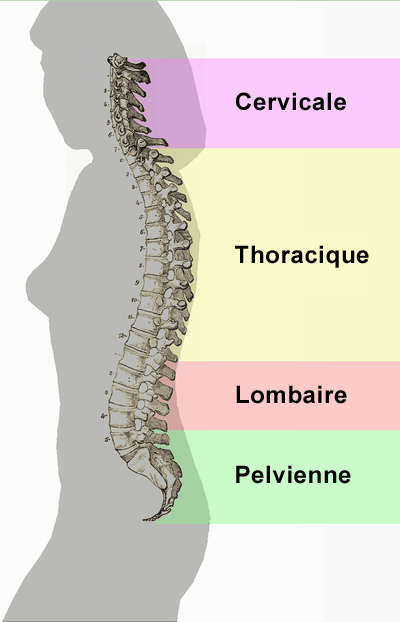
\includegraphics[width=0.4\linewidth]{Figures/rachis.png}
	}
	\caption{Régions de la colonne vertébrale humaine. Tiré de \cite{rachisWiki} sous la licence Creative Commons.}
	\label{fig:rachis}
\end{figure}

La hauteur de la lésion s'exprime donc en fonction de la vertèbre correspondante. La hauteur de la lésion influe sur les conséquence de celle-ci. En effet, plusieurs nerfs sortent de la moelle épinière à chaque vertèbre. Ainsi une coupure de la moelle épinière entraînera une perte de connexion nerveuse pour tous les nerfs situés en dessous de la lésion. Il en résulte que plus la lésion est haute, plus l'incapacité qui en résulte est grande. 

Le projet portant principalement sur les personnes BM de haut niveau, les conséquences d'une lésion entre C1 et C8 seront présentées plus en détails. Le tableau \ref{tab:hauteurlesion} présente les conséquences motrices et sensorielles d'une lésion médullaire au niveau des vertèbre cervicale en fonction de la vertèbre touchée \citep{apparelyzed2008}.

\begin{table}[ht]
	\caption{Conséquence motrices en fonction de la hauteur de la lésion médullaire.}
		\begin{tabular}{|c|c|}
		\hline
	    	 	C7 - C8 & Mouvements complets du cou et de la tête \\
	    	 	& Bons mouvements des épaules\\
	    	 	& Système nerveux parasympathique compromis, Possibilité d'hyperréflexie autonome\\
	    	 	& Paralysie complète du tronc et des jambes\\
	    	 	& Mouvement partiel des doigts, bons mouvement du reste du bras\\
	    \hline
	    	 	C6 & Aucun mouvement des doigts, pas d'extension du coude ni de flexion du poignet\\
	    \hline
	    		C5 & Aucun mouvement du poignet\\
	    	\hline
	    		C4 & Mouvements du cou dépendamment de la force musculaire résiduelle \\
	    		& Mouvements limités des épaules\\
	    		& Aucun mouvement du coude\\
		\hline
			C1 - C3 & Mouvements de la tête limités en fonction du tonus musculaire résiduel\\
			 & Paralysie complète des bras\\
			 & utilisation des muscles du thorax et diaphragme pour respirer impossible\\	    
	    \hline
		\end{tabular}
	\label{tab:hauteurlesion}
\end{table}

La deuxième caractéristique de la lésion est son type. Celle-ci peut être soit complète, soit incomplète. Une lésion complète correspond à une coupure nette de toute conduction nerveuse située en dessous de la lésion, tandis qu'une lésion incomplète peut, suivant la lésion conserver les conductions nerveuses passant dans la partie de la moelle épinière non lésée.

Le tableau \ref{tab:typelesion} présente les quatre grands types de lésions médullaires incomplète et leurs conséquence sur les pertes sensorielles et motrices qui en résultent \citep{apparelyzed2008}.

\begin{table}[ht]
	\caption{Types de lésions de la moelle épinière et conséquences.}
		\begin{tabular}{|c|c|}
		\hline
	    	 	Syndrome cordonal antérieur & Partie frontale de la moelle épinière endommagée\\
	    	 	& Perte de sensation de douleur, toucher et chaleur\\
	    	 	& Possibilité de retrouver un mouvement plus tard\\
	    \hline
	    	 	Syndrome cordonal postérieur & Partie dorsale de la moelle épinière endommagée\\
	    	 	& Conservation du tonus musculaire et des sensations \\
	    	 	& Perte de coordination des mouvements des membres\\
	    \hline
	    		Syndrome cordonal central & Centre de la moelle épinière endommagé\\
	    		& Perte de l'usage des bras\\
	    		& Conservation possible de certaines fonctions des jambes\\
	    		& Contrôle des intestins et de la vessie possible \\
	    		& Guérison progressive possible\\
	    	\hline
	    		Syndrome de Brown-Séquard & Dommages concentrés sur un côté seulement de la moelle \\
	    		& Perte de mouvement du côté de la lésion mais conservation des sensations\\
	    		& Perte des sensation du côté opposé mais conservation des mouvements\\
	    \hline
		\end{tabular}
	\label{tab:typelesion}
\end{table}

Au regard de ces informations, on peut déduire que chaque personne aura besoin d'une assistance spécialisée dépendant du type de sa lésion et de sa hauteur. Le BM de niveau C1-C3 seront complètement dépendant, et auront même besoin d'une aide à la respiration. 

De même que pour se déplacer et réaliser les action de la vie quotidienne, ces personnes nécessiteront des aides. Ces aides sont présentées dans la partie suivante.

\section{Les aides techniques aux actions de la vie quotidienne (AVQ)}

Chaque BM a un profil singulier en fonction de la hauteur de sa lésion et de la nature de celle-ci. Ceci implique que chaque personne aura besoin d'une aide particulière pour l'aider à vivre au quotidien. Pour ce faire,  l'avancée de la technologie dans le domaine de la santé a permis de concevoir des appareil améliorant grandement les conditions de vie de ces personnes. Ces appareils sont appelés les aides techniques. 

\subsection{Les aides techniques en général}

Les aides techniques se présentent sous beaucoup de forme, et peuvent être très simples comme un simple crochet pour attraper des objets, comme très complexes comme par exemple un bras robotique manipulateur. On retrouve une diversité d'objet ayant tous pour but de venir en aide aux personnes dans leurs AVQ, que ce soit, pour s'habiller, se déplacer, se nourrir, se laver, se lever ou communiquer. Les matelas anti-escarres, les orthèses et les bas de contention sont également considérés comme des aides techniques.

Notre étude se concentrera sur les aides techniques en rapport avec le projet, à savoir les fauteuil roulants motorisés (FRM) et le bras manipulateur Jaco.

Les FRM sont une des aides techniques les plus importantes pour les personnes paralysées, car elle leur permet de pouvoir se déplacer de manière autonome ou presque (le transfert dans le fauteuil devant être assisté). Toute fois, suivant le niveau de lésion d'un BM, celui-ci pourra ne pas être en mesure de s'en servir efficacement. En effet, un BM de niveau suppérieur à C6 ne pourra pas se servir d'un \textit{joystick}, du fait qu'il ne possède plus de mouvement résiduel dans les doigts. 

Pour palier ce problème, les concepteurs d'aides techniques ont du mettre au point des méthodes de contrôle de ces aides adaptées au personnes n'ayant plus l'usage de leur mains. Ainsi, des manettes de contrôles ont été rajoutées sur les côtés de la tête, activées lorsqu'elles sont poussées par l'action du cou. Un contrôle par le souffle a également été inventé, grâce à un tube placé devant la tête de la personne, dans lequel celle-ci pourra souffler ou aspirer.

Ces faits dénotent une volonté de diversifier les interfaces de contrôle des aides technique afin qu'un maximum de personne puisse les utiliser efficacement.

\subsection{Le bras manipulateur Jaco}

\begin{figure}
	\centering
	\fbox{
		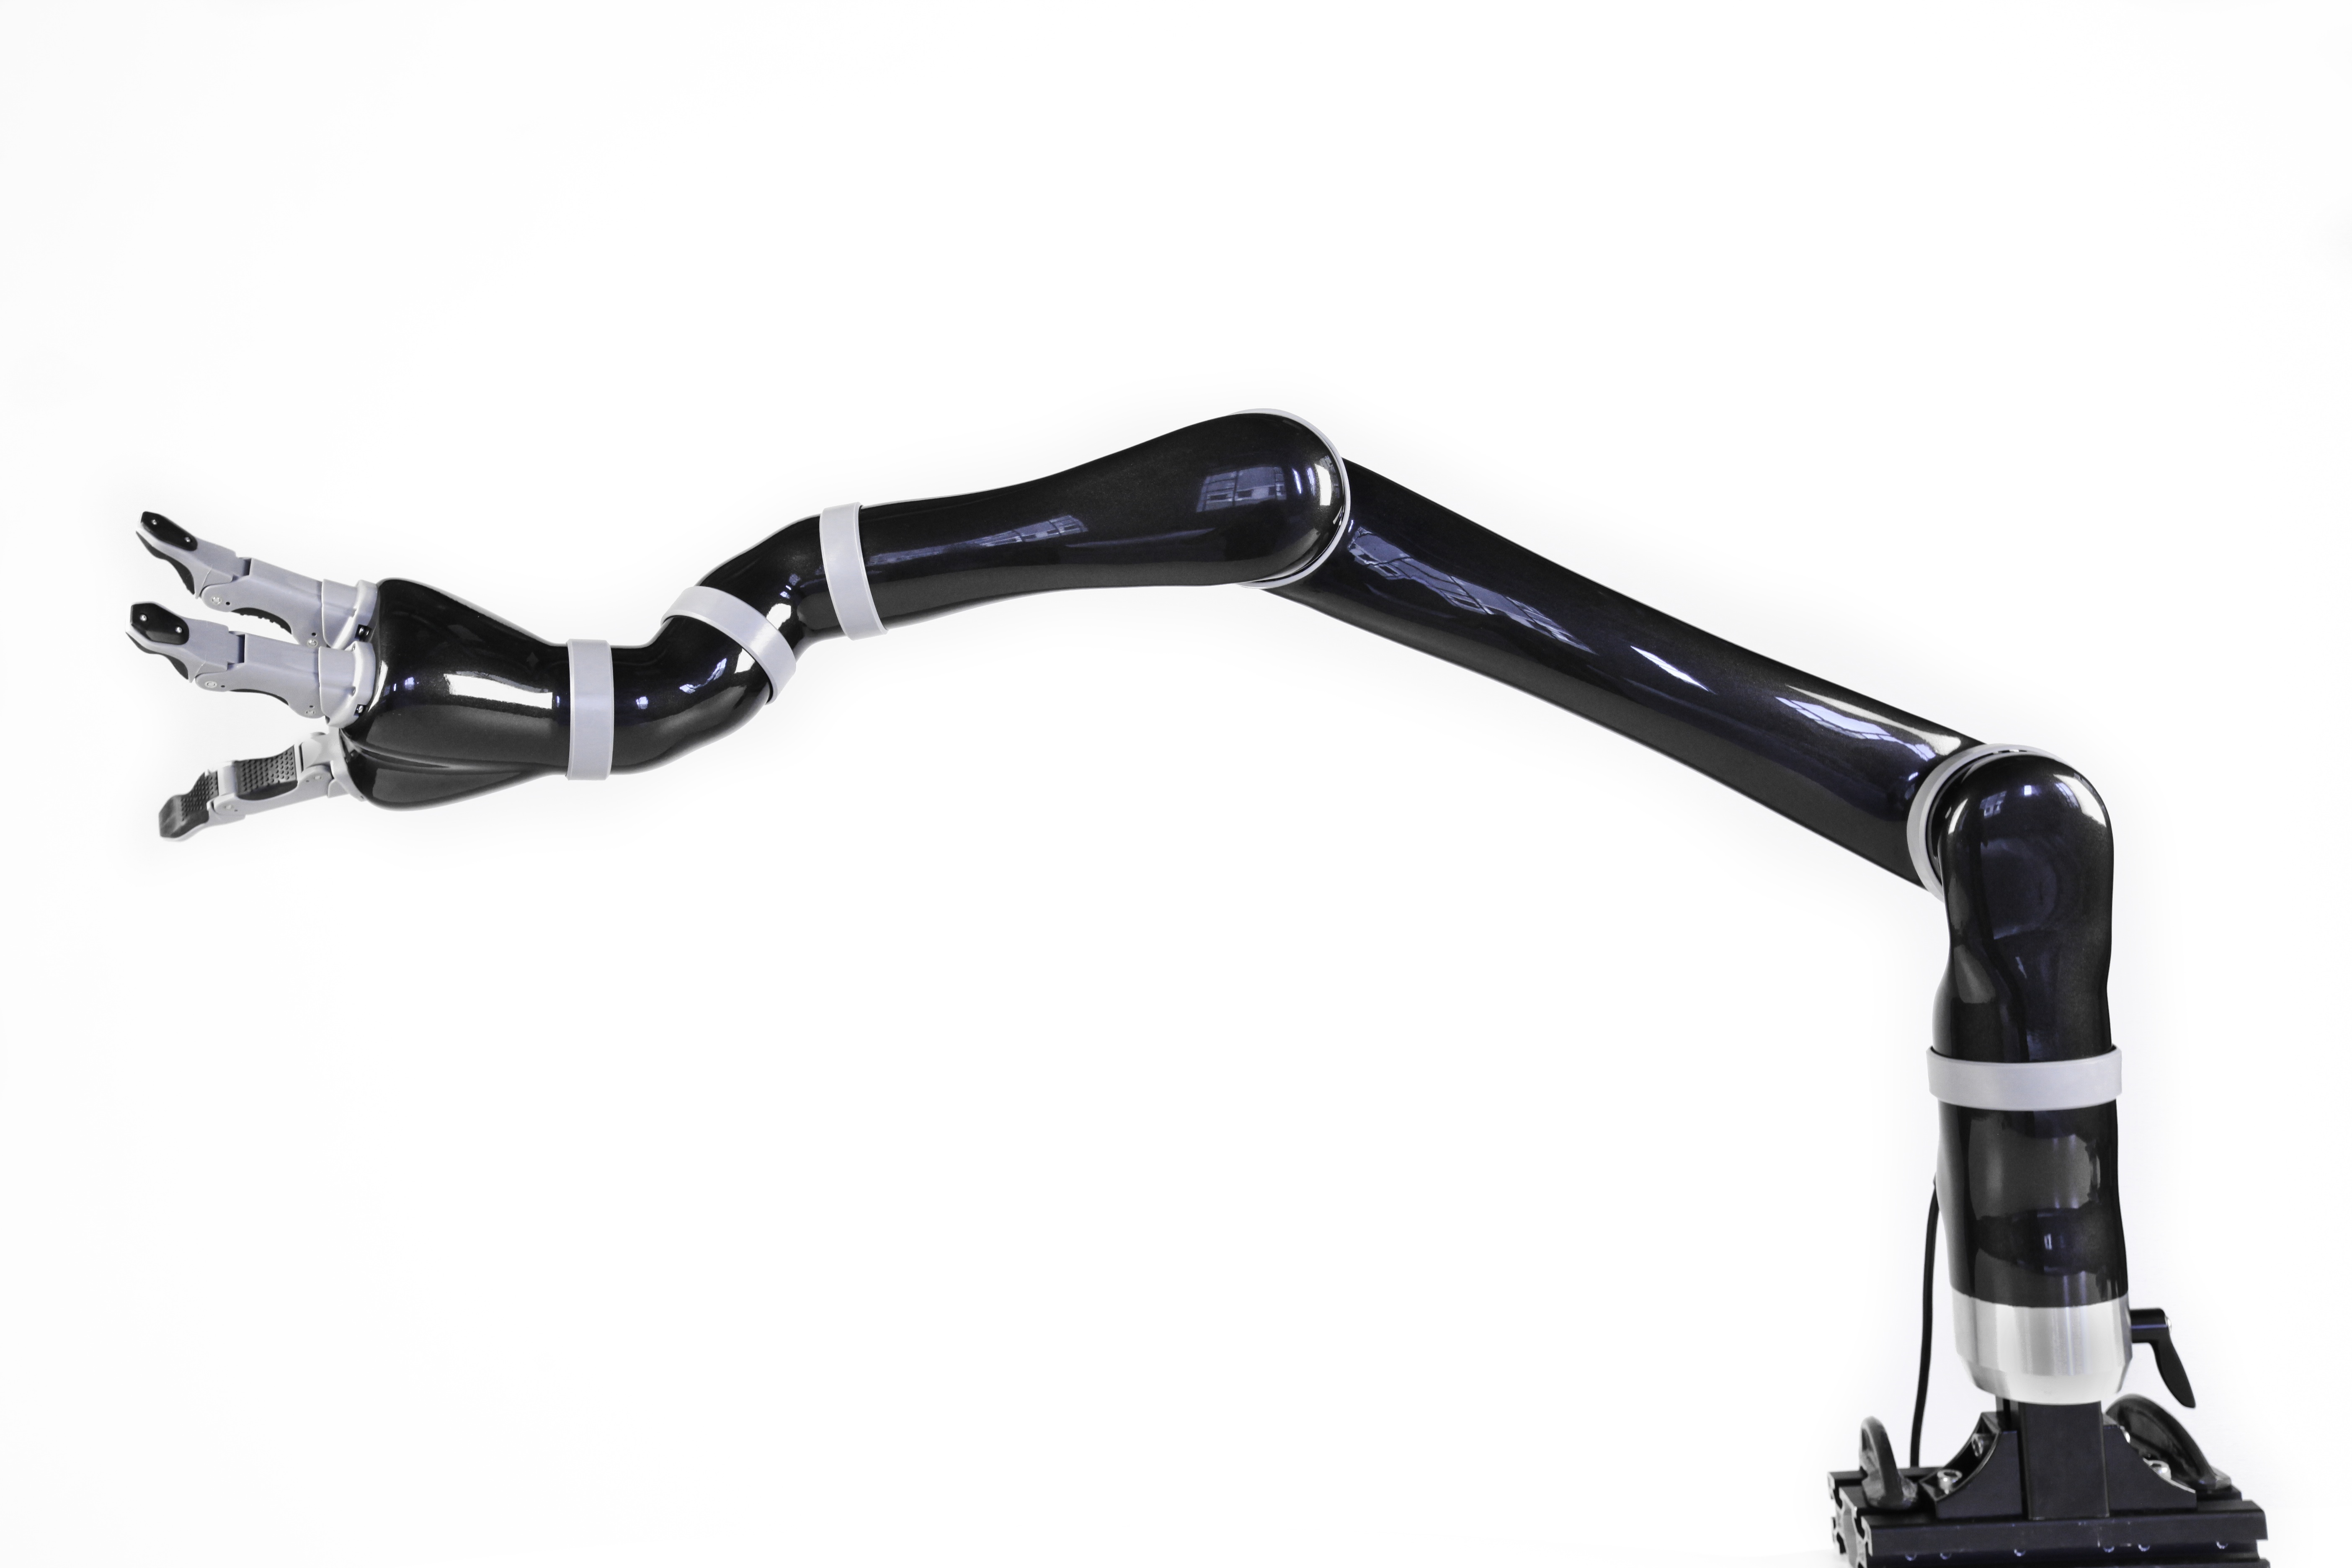
\includegraphics[width=0.8\linewidth]{Figures/jacofull.jpg}
	}
	\caption{Bras manipulateur Jaco, tiré de \cite{Kinova2012} avec l'autorisation de Kinova}
	\label{fig:jacofull}
\end{figure}

Jaco (figure \ref{fig:jacofull}) est un bras robotique manipulateur conçu par la société canadienne Kinova depuis 2006, et a pour but d'aider les personnes en FRM dans leurs AVQ. Il est conçu pour être monté directement sur le FMR d'une personne et est contrôlable à l'aide d'un \textit{joystick}.

Le bras pèse au total 5.7 Kg, a un rayon d'action de 90 cm et peut porter une charge allant jusqu'à 1.5 Kg lorsque le bras est en demi-extension et 1 Kg lorsqu'il est en extension complète. Il est composé de 7 degrés de liberté (DDL) lui permettant toutes les combinaisons de translations et rotations dans l'espace et possède une main articulée de 3 doigts permettant la saisie de petits objets.

L'utilisation principale de ce robot réside donc dans la préhension d'objets, l'ouvertures de portes, permettant ainsi à une personne en fauteuil roulant et sans usage de ses bras de se déplacer chez lui, de boire et de manger.

Le \textit{joystick} du bras possède trois axes et plusieurs bouton afin de contrôler tous les mouvements possible. De ce fait, une bonne dextérité est nécessaire pour l'utiliser efficacement, ce qui pause problème aux personnes BM de haut niveau.

Jaco est également livré avec une suite logicielle intégrée permettant de configurer le bras grâce à une liaison USB. Une bibliothèque de programmation est également fournie. Celle-ci permet de contrôler Jaco et de récupérer les informations générée par celui-ci dans un programme externe, conçu par l'utilisateur. 

Cette solution permet une grande liberté et ouvre la possibilité à tout un chacun de pouvoir développer une nouvelle méthode de contrôle pour le bras.

\section{Le Signal Électromyographique (EMG)}

L'électromyographie consiste en l'acquisition de l'activité électrique présente sur un muscle lors de sa contraction. Le signal peut être acquis en surface grâce à une électrode collée directement sur la peau au dessus du muscle, ou directement à l'intérieur du muscle de manière invasive à l'aide d'une aiguille.

Le signal généré par un muscle s'exprime en millivolts (mV) et permet l'analyse de l'activité musculaire d'une personne. L'EMG est utilisé surtout en médecine pour la détection de problèmes liés au système nerveux chez un patient.

Le mécanisme de contraction musculaire part du système nerveux central qui envoie un signal nerveux de contraction volontaire à un muscle. Ce signal est transporté jusqu'aux muscles en passant par la moelle épinière puis par un nerf moteur. C'est ce nerf moteur qui transmet le potentiel électrique à chaque fibre musculaire présente dans le muscle. 

Chaque fibre musculaire est alors parcourue par un potentiel d'action tel que décrit sur la figure. Les fibres musculaires actionnées lors d'un mouvement sont recrutées aléatoirement et change à chaque mouvement. Ce mécanisme permet de retarder la fatigue musculaire en répartissant la charge sur des fibres différentes.

Le signal EMG généré est constitué de la somme de tous les potentiels d'action musculaires des fibres recruté pour le mouvement et se présente comme sur la figure \ref{fig:emg}.
%TODO : ajouter figure EMG


\chapter{Revue de Littérature}

La classification de mouvements grâce au signal EMG a été énormément étudiée dans la littérature. Toute fois, une partie seulement de ces études l'a traitée de manière temps réelle. Enfin un type d'application vient encore se démarquer dans ce sous ensemble : les applications embarquées. 

Par application embarquée, nous entendons un système fonctionnant de manière autonome sur une carte électronique pouvant être déplacée facilement. Il faut donc enlever a ce sous ensemble toutes les applications réalisées sur ordinateurs. 

La première partie de cette revue de littérature s’intéressera à la classification EMG en temps réel, tandis que la deuxième partie sera centrée sur les applications embarquées dont fait état la littérature dans son état actuel.

\section{Classification EMG}

L’analyse des signaux EMG et la détermination du mouvement effectuée à partir de ceux-ci se divise en plusieurs grandes sous-parties incluant chacune un algorithme bien précis. Chacune de ces parties peut être réalisée avec plusieurs algorithmes différents impliquant chacun une précision, et une facilité d’implémentation différente. Des compromis doivent donc être faits entre la précision engendrée par un algorithme et sa complexité d’implémentation et d’exécution qui est souvent inversement proportionnelle. 

La première étape de traitement des signaux EMG consiste à déterminer quand il y a une activité musculaire et quand il n’y en a pas. Celle-ci est appelé détection d’activité, ou détection d'onset, et c’est la première partie qui sera analysée. L’étape suivante est l’extraction des caractéristiques du signal qui pourront permettre ensuite au classificateur de déterminer quel mouvement a été effectué. Enfin, une analyse de différents classificateurs sera effectuée, se basant sur les mêmes critères que les autres algorithmes, à savoir la précision, la facilité d’implémentation et le temps d’exécution. 

Un point important est à souligner, et ce point constituera un premier point de cette étude : tous ces algorithmes mis bouts à bouts doivent, une fois le choix d’architecture effectué permettre de réaliser le traitement de quatre canaux EMG en temps réel.

\subsection{Fenêtrage du signal}

Le signal électromyographique est découpé à des fins d'analyses et pour extraire les caractéristiques de celui-ci. La longueur de ces fenêtres est exprimée en temps ou en nombre d'échantillons. Un pas d’incrément est également défini, afin de choisir si les fenêtres se recouvrent ou non. 

La littérature étudiée fait état de beaucoup de tailles de fenêtres et de pas d’incréments différents. La plupart sont fixés de manière heuristique. Cependant, \cite{Englehart2003} évoquent le fait que cette fenêtre ne doit pas être trop grande de manière à ce que le temps de cette fenêtre et de son temps de traitement n’excède pas les 300ms de latence maximum au-delà desquels la latence est ressentie par l’utilisateur. Ainsi, leur fenêtre est fixée à 250ms avec un pas d’incrément à 125ms de manière à garder une marge suffisante pour le temps de calcul. 

Une fenêtre trop petite est sujette au biais de variance généré par les variation du signal et de ces caractéristiques qui peuvent jouer sur la précision du classificateur utilisé.

Un compromis doit donc être fait sur la longueur des fenêtres utilisées entre la  précision du classificateur et son temps de réponse.

\subsection{Algorithmes de détection d'activité}

Une fois une fenêtre du signal acquise, la première étape est la détection d'activité musculaire, ou détection d'"onset". 

La détection d’onset est le principe qui consiste à détecter le début d’une activité musculaire sur le signal EMG de manière automatique.  Pour ce faire, plusieurs algorithmes semblent bien fonctionner en combinant à la fois, une bonne précision et un nombre d’opérations flottantes à réaliser restreint. Cette détection d’onset permet d’économiser les ressources processeurs afin  de n’extraire les caractéristiques du signal que lorsque c’est utile et surtout de délimiter les zones d’activité musculaire pour la détection de mouvement. 
Il existe ainsi plusieurs caractéristiques du signal qui peuvent être extraites afin de détecter un onset. Une première largement utilisée \citep{Chang1996, Englehart2003, Tenore2007}est la méthode du Zero Crossing Rate (ZCR). Elle calcule le nombre de fois où la courbe du signal repasse par zero. 

Un élément important est que \cite{Chang1996} ont développé cette méthode sur un DSP et semble fournir des résultats satisfaisants. Cette étude présente également la mise en place d’une dead zone sur l’algorithme de zero crossing, qui permet de réduire, voir de supprimer l’influence du bruit sur le ZCR.
Le ZCR est une méthode simple à implémenter et très peu couteuse en ressources processeur pour la raison qu’elle ne nécéssite qu’un nombre d’addition égal N-1, N étant le nombre d’échantillons dans la fenêtre analysée. 

\cite{Peleg2002} optent pour une méthode consistant à appliquer un seuil directement sur l’enveloppe du signal. Le signal est d’abord passé dans un filtre passe-haut à 30Hz, puis la valeur absolue du signal est faite, enfin, le signal est passé dans un filtre passe-bas à 2.5Hz. Cette méthode est une analogie de la méthode Mean Absolute Value (MAV), le filtre passe bas ayant pour but d’effectuer une moyenne des valeurs absolues du signal. Suite à cela, le seuil appliqué sur l’enveloppe est fixé comme étant 10 pourcents plus haut que la valeur de l’enveloppe de l’EMG au repos. 

\cite{Tenore2007} utilisent également la méthode MAV sans toutefois préciser la manière dont ils ont choisi leur seuil de détection. 

Une autre méthode simple à implémenter et peu couteuse en temps de calcul est la méthode de la Teager-Kaiser Energy (TKE) qui correspond à un taux de variation du signal. Elle a été utilisée par \cite{Maheu2011} comme une caractéristique du signal utilisée dans la classification, mais peut aussi être utilisée dans la détection d’onset comme l'ont montré \cite{li2007}. Elle ne constitue qu’une soustraction et deux multiplications par échantillon dans la fenêtre d’analyse. 

\subsection{Caractéristiques du signal EMG utilisées}

Une fois l’ctivité musculaire du signal EMG détectée, on cherche à déterminer quel mouvement a été effectué. Ce travail est effectué par un classificateur. Ce classificateur doit donc prendre des éléments de comparaison en compte pour déterminer l’action faite. Ces éléments doivent être significatifs du signal capté, et sont appelés des features, ou des caractéristiques. 
Les caractéristiques extraites des signaux EMG sont nombreuses, aussi nous nous concentrerons sur celles ayant les meilleurs résultats dans la littérature. Ainsi la caractéristique ayant le plus de succès semble être l’auto-régression \citep{Chang1996, Peleg2002, Maheu2011}.

L’auto-régression consiste à trouver les n+1 coefficients d’un polynôme d’ordre n qui, appliqué sur un signal aléatoire, permettra de retrouver une approche du signal réel. Plusieurs algorithmes permettent de retrouver ces coefficients autorégressifs (AR).

\cite{Peleg2002} utilisent une auto-régression d’ordre 11. Cet ordre « a été déterminé de manière heuristique » \citep{Peleg2002}.

\cite{Chang1996} ont choisi l'utilisation des coefficients AR mais également les coefficients cepstraux obtenus à partir des AR. Ils préconisent également de fixer l’ordre de l’AR à 4 en se basant sur la littérature et en justifiant par un compromis entre une bonne représentation du signal  et un temps de calcul court. 
L’obtention des coefficients cepstraux à partir des coefficients AR se fait grâce à une relation mathématique récursive simple dépendant de l’ordre de l'auto-régression réalisée. 


\subsection{Classificateurs utilisés dans la détection de mouvements}

Une fois les caractéristiques du signal calculées,  celles-ci sont entrées dans un classificateur qui, grâce à un apprentissage, permet de déterminer quel mouvement a été effectué par le sujet. Encore une fois, beaucoup d’algorithmes existent pour réaliser cette opération. Toutefois, beaucoup de ceux-ci sont très consommateurs en temps de calculs, comme les réseaux de neurones (RN), où les analyses linéaires discriminantes (LDA). 

Toute fois \cite{englehart1999} ont montré que l'importance du choix du classificateur pour la reconnaissance de mouvements à partir de signaux EMG est limitée et que les gains en termes de performances de classificateurs complexes tels que les RN sont négligeables par rapport aux performances d'un classificateur plus simple comme le LDA.

Ceci étant dit nous nous intéresserons donc plus particulièrement aux deux études principales mettant en œuvre des dispositifs temps réels embarqués.

\cite{Chang1996} utilisent dans leur application embarquée un algorithme utilisant les distances des maximums de vraisemblances (MMLD), tandis que \cite{Tenore2007} utilisent quant à eux un classificateur de type LDA.


\section{Systèmes Embarqués temps réels et EMG}

La littérature comprend très peu d'applications embarquées de traitement temps réel de signaux EMG. Ainsi un premier article de référence a été publié par \cite{Chang1996} et rapporte la réalisation du traitement de 4 électrodes EMG afin de contrôler un pointeur informatique dans le but de remplacer une souris. Cette étude fait référence dans notre projet car elle a été développée dans le but de venir en aide aux blessés médullaires de haut niveau. 

Deux études de la même époque traitent ensuite également de traitement embarqué des EMG. \cite{martinez1999} utilisent un dsp, sans toutefois préciser lequel, pour traiter un canal EMG tandis \cite{Prasad1996} ont conçu une carte à base de DSP implantée dans un ordinateur pour acquérir et traiter cinq canaux EMG.

Enfin l'étude la plus récente est celle de \cite{Tenore2007} qui présentent dans leur article avoir réalisé l'une des premières applications embarquées classifiant le signal EMG.

\subsection{Le traitement temps réel}

Le temps réel au sens strict du terme en informatique, signifie que l’on doit savoir à tout instant combien de temps prendront les différentes actions réalisées par un programme. Ce temps peut s'exprimer de plusieurs manières, les deux principales étant le temps en secondes et le nombre d'instructions élémentaires d'une unité de calcul (microprocesseur, microcontrôleur).

Dans notre cas, et comme fixé dans la littérature du contrôle par EMG, la contrainte principale est le temps de réaction et de calcul maximal à laquelle le système doit satisfaire. La littérature traitant de l’implémentation temps réelle de tels systèmes parle ainsi d’un délai de calcul maximal de 300 millisecondes afin que l’utilisateur humain ne ressente pas la latence du système \citep{Chu2007, Englehart2003}.

\subsection{Méthodes d'acquisition du signal}

La plupart des études utilisées pour cette revue utilisent des électrodes de surface pour faire leur reconnaissance de mouvements. Cependant, les manières de filtrer et d'échantillonner sont différentes à travers les études. Cette partie a pour but de les regrouper et de les comparer. 

La plupart des études observent une fréquence d’échantillonnage de 1KHz permettant d’obtenir une bande utile théorique (respectant le théorême de Shannon) pour les signaux EMG allant jusqu’à 500Hz \citep{Chang1996, Chu2007, Englehart2003, Tenore2007}. 
La plupart des signaux EMG bruts sont amplifiés avec des gains de l’ordre de 2000, sont passé dans des filtres passe bande entre 10 et 450 ou 500 Hz.

\cite{Peleg2002} ont toutefois opté pour une fréquence d’échantillonnage à 500Hz, avec un filtre anti repliement à 250Hz, alors que \cite{Crawford2005} ont opté pour une fréquence d’échantillonnage à 2048 Hz.
Lorsqu’elles sont mentionnées, la précision des ADC utilisés varie suivant les études, allant de 16 bits \citep{Englehart2003} à 12 bits \citep{Tenore2007, Fukuda2003, Prasad1996}.


\subsection{Matériel informatique utilisé dans la littérature}

La plupart des application trouvées dans la littérature n'ont pas une définition toujours précise de la notion de temps réel. La plupart des articles présentent un système exécuté sur des machines puissantes, sur des systèmes d'exploitation souvent non temps réels. 

\cite{Englehart2003} ont réalisé une implémentation temps réelle d’algorithmes de reconnaissance de mouvement à partir de signaux EMG. Cette réalisation a été réalisée sous matlab et son extension de programmation temps réel sur un PC distant.

Si l'on s'interesse plus particulièrement aux applications embarquées, \cite{Chang1996} ont réalisé un montage électronique basé sur un DSP TMS320C31 de chez Texas Instruments. C’est un processeur 32bits comprenant un cœur à virgule flottante tournant à une fréquence de 20MHz, avec quatre niveaux de pipe-line permettant d’exécuter une instruction à chaque cycle d’horloge. Cette architecture leur a permis d’obtenir un temps total de traitement du signal entre 140 et 160 ms ce qui satisfait à la condition évoquée au début de l’étude concernant le respect d’un temps de réponse maximum de 300 ms. Toutefois, cette étude ayant été réalisée en 1996, il existe aujourd’hui quantité de DSP plus rapide et plus efficaces.

Toute fois cette étude, ainsi que celles de \cite{martinez1999} et de \cite{prasad1996} ont aujourd'hui autour d'une quinzaine d'années et le matériel informatique utilisé alors a aujourd'hui beaucoup évolué.

\cite{Tenore2007} ont utilisé également un DSP de chez Texas Instruments : un TMS320VC5509A couplé à un ADC dédié de chez National Instruments. Ce DSP est un processor comprenant un cœur à virgule fixe exécutant des actions relativement simples, comme le calcul du ZCR du signal, le calcul de la longueur d’onde du signal et le MAV. Ce DSP leur a permis d'implémenter un classificateur LDA.

\chapter{Problématique et Objectifs du Projet}

Aujourd'hui, l'avancée des technologies dans le domaine de la santé a permis de gros progrès médicaux, y compris dans le domaine de la réadaptation et de l'aide à la personne. Cette avancée a permis la conception d'aides techniques de plus en plus évoluées et capable d'améliorer sensiblement les condition de vie des personnes dépendantes, et plus particulièrement des blessés médullaires. 

Cependant, les personnes les plus sévèrement touchées par des blessures de la moelle épinières ne peuvent profiter de certaines de ces avancées, car elles n'ont plus la capacité de se servir de ces aides efficacement. 

Connaissant ces paramètres, la société Kinova produisant le bras robotique manipulateur Jaco, a décidé de développer une nouvelle interface de contrôle de Jaco afin que des personnes ne possédant plus l'usage de leurs doigts soient capable d'exploiter le potentiel du robot.

Pour cela, l'utilisation du signal EMG a été préconisée à la suite du projet de maîtrise \cite{Maheu2011}, aujourd'hui employée de Kinova. L'enjeu de ce projet est donc en grande partie économique pour la societé Kinova, qui sera alors en mesure d'élargir sont panel de clients potentiels.

L'étude de la littérature a également permis de constater que les applications de contrôles par EMG en temps réel étaient rares et encore plus lorsqu'on en vient à parler d'application embarquée.

Ceci permet ainsi d'ajouter un enjeu purement scientifique au projet en participant à l'avancée scientifique du monde des technologies de la santé.

Les objectifs du projet sont les suivants : 

\begin{itemize}
 \item Réaliser un prototype embarqué capable de reconnaître le mouvement effectué par l'utilisateur en temps réel et en utilisant les signaux EMG de la personne.
 \item Respecter la contrainte temps-réelle fixée par la littérature de 300ms
 \item Effectuer un traitement simultané de quatre canaux EMG
 \item Appliquer une commande sur le bras robotique Jaco en fonction du mouvement détecté
\end{itemize}

Le but principal n'est pas la réalisation d'un produit fini, mais l'établissement d'une preuve de concept pour cette application. La réalisation doit donc permettre de dire si la réalisation d'un tel produit est faisable ou non, et quels choix sont préconisés pour ce faire.

Le projet est réalisé en partenariat avec le CRSNG et la société Kinova sous la forme d'un projet ENGAGE. 

\chapter{Méthodologie}
\label{CHmethodo}

\section{Choix des Muslces}

Le premier choix important est de choisir quels muscles seront utilisés pour réaliser la commande. Dans un premier temps, le critère principal est que les muscles choisis doivent toujours être fonctionnels chez les blessés médullaires. Ainsi, les muscles choisis par \cite{Chang1996}, les trapèzes et les sterno-cléïdo mastoïdiens sont considérés comme un choix judicieux dans un premier temps. En effet, ces deux muscles sont innervés en partie par des nerfs passant par la seconde vertèbre cervicale, ainsi, la plupart des blessés médullaires conserveront au moins une activité résiduelle dans ces muscles. 

\begin{figure}
	\centering
	\fbox{
		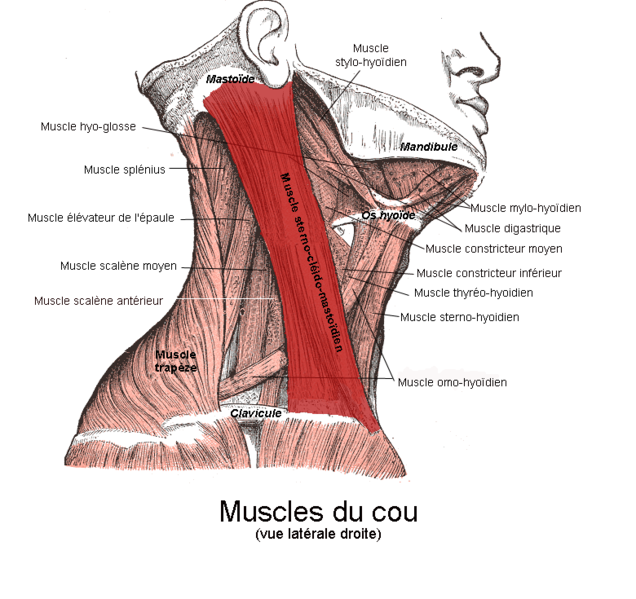
\includegraphics[width=0.6\linewidth]{Figures/muscles.png}
	}
	\caption{Muscle sterno-cléïdo mastoïdien et muscles du cou.Tiré de \cite{sternoWiki} sous la licence Creative Commons.}
	\label{fig:muscles}
\end{figure}


Un autre muscle à considérer serait également le muscle occipito-frontal qui opère l'élévation des sourcils. Toute fois, il est peu probable que les personnes blessées médullaires apprécient le fait d'avoir des électrodes collées sur le front en permanence. Ce muscle ne représente donc pas une alternative viable pour le projet, de même que pour tous les autres muscles faciaux.

Une autre solution serait d'utiliser les muscles fléchisseurs et extenseurs du poignet. Toute fois, ces muscles sont innervés respectivement par les nerfs médian et radial dont les faisceaux passent par les dernières vertèbres cervicales ainsi que la première vertèbre thoracique. Ainsi, les blessés médullaire de haut niveau n'auront plus suffisamment, voir plus du tout d'activité résiduelle dans ces muscles.

Un point vient également appuyer la sélection des muscles trapèzes et sterno-cléïdo mastoïdiens et qui va influencer la manière de développer le projet : l'acquisition de signaux EMG sur ces muscles n'implique pas de "cross-talk" c'est à dire qu'on ne voit pas l'activité d'un muscle sur l'enregistrement des autres. Cette observation a été réalisée au début de la réalisation du projet, après avoir effectué des tests préliminaires. Ainsi, en faisant des mouvements simples de rotation de la tête et d'élévation des épaules, on ne voit qu'un seul muscle s'activer. Cette considération permet de faire un choix drastique sur la complexité du projet : on choisit de ne monitorer que des mouvements unitaires simples n'activant qu'un seul muscle. 

Ainsi, on est capable d'établir un lien direct entre l'activité musculaire d'un muscle particulier et le mouvement réalisé. Lorsqu'une activité est détectée sur un muscle sterno-cléïdo mastoïdien, c'est qu'une rotation de la tête a été effectuée, et si une activité est détectée sur un trapèze, c'est une élévation de l'épaule qui a été réalisée.

Ce postulat permet de réduire le temps de calcul nécessaire au traitement des signaux en enlevant complètement l'étape de classification. Ce choix comporte des points négatifs et des points positifs. Un atout majeur est de retirer toute la charge de calculs nécessaire pour le classificateur, et de concentrer ces calculs sur la détection d'activité musculaire ainsi que sur le filtrage numérique du signal. En contrepartie, le nombre de mouvements reconnus par le systèmes est réduit à quatre mouvements unitaires : un pour chaque muscle. 

Cependant cette perte en diversité de mouvements pourra être en partie comblée par des stratégies de communication différentes pour ces mouvements. En effet, on pourra effectuer des mouvements prolongés ou bien des mouvements composés de plusieurs activations courtes répétées. Ces stratégies permettront d'étendre la diversité de commande tout en ne reconnaissant que quatre mouvements. 


\section{Architecture Matérielle}\label{CHarchimat}

Une fois le choix des muscles arrêté, les premiers choix a effectuer seront les choix architecturaux, et dans un premier temps, ceux concernant l'architecture matérielle. Ce chapitre présente les choix matériels effectués pour la conception du système tout en argumentant pourquoi chaque choix a été effectué et dans quel cadre.

\subsection{Électrodes}

Le choix des électrodes est une phase importante du projet car leur choix détermine la charge de travail qui va en résulter. En effet, des électrodes donnant un signal brut, très faible (la tension d'un signal EMG étant de l'ordre du millivolt) est impossible a exploiter tel quel et nécessite des étape de filtrage et d'amplification avant de pouvoir être échantillonné. Ainsi choisir ce type d'électrode ajoute une étape de conception électronique supplémentaire afin que le signal soit exploitable.

Le LIO travaille depuis maintenant plusieurs années avec des électrodes construites par la compagnie Delsys : les électrodes DE-2.3 et se présentent comme sur la figure \ref{fig:de2.3}. 

\begin{figure}
	\centering
	\fbox{
		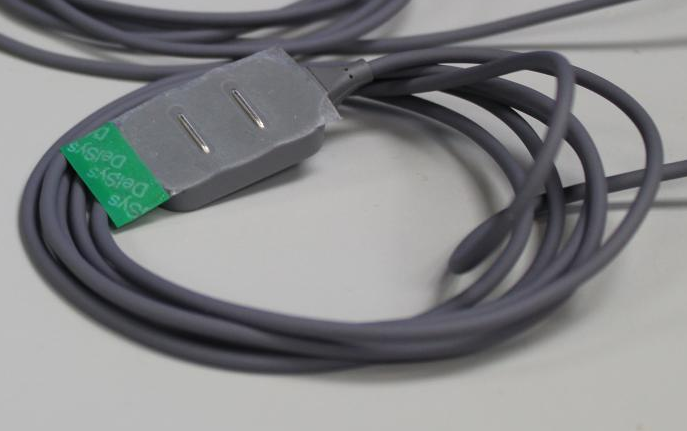
\includegraphics[width=0.42\linewidth]{Figures/de23.png}
	}
	\caption{Électrode Delsys DE-2.3.}
	\label{fig:de2.3}
\end{figure}

Ces électrodes, contrairement au modèle moins cher DE-2.1 sont pré-amplifiées avec un gain de $1000 V/V \pm 1\%$ et pré-filtrées sur une bande passante de $20-450 Hz \pm 10\%$. Ceci nous permet de limiter les étapes de filtrage analogique avant de faire entrer le signal de l'électrode dans le microcontrôleur. En effet, le filtrage passe-bande déjà présent permet de garder la bande utile du signal EMG tout en limitant le bruit d'échantillonnage.

Les électrodes sont câblées avec du fil blindé, protégeant des interférences électromagnétiques, le blindage étant relié à la masse du circuit. Pour que ce blindage soit efficace, le connecteur utilisé doit être également de bonne qualité. Pour ce faire, des connecteurs de marque LEMO sont utilisés. Ces connecteurs sont utilisés dans beaucoup de domaines critiques demandant des connecteurs résistants au temps et aux interférences. 

Ainsi les connecteurs LEMO femelles correspondant à ceux présents sur les câbles des électrodes ont été acquis afin de relier les électrodes au système.

\begin{figure}
	\centering
	\fbox{
		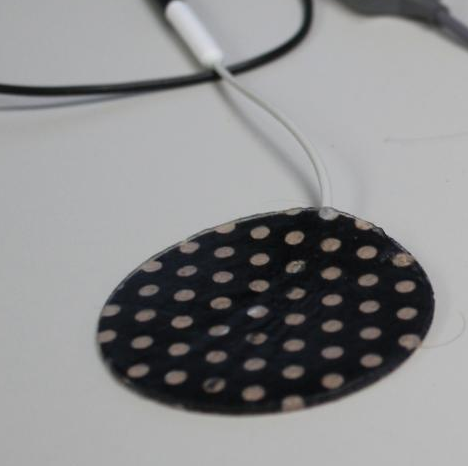
\includegraphics[width=0.42\linewidth]{Figures/delsysneutre.png}
	}
	\caption{Électrode Delsys neutre.}
	\label{fig:delsysneutre}
\end{figure}

Plusieurs électrodes neutres, comme présentées par la figure \ref{fig:delsysneutre}, ont également été acquises. Ces électrodes sont nécessaires car c'est la référence utilisée pour mesurer la tension acquise sur les muscles. Elles seront positionnées sur une partie la moins charnue possible, comme par exemple la pointe du coude de l'utilisateur. Elles seront connectées directement à la référence du convertisseur analogique-numérique du microcontrôleur.

\subsection{Microcontrôleur}\label{ch:microcon}

Le deuxième choix matériel important concerne celui du microcontrôleur ou du contrôleur de signaux numériques (DSP). En effet, ce choix est déterminant car c'est lui qui opèrera tous les calculs nécessaires au bon fonctionnement du système. Son choix est donc à faire de manière réfléchie. 

Avant de présenter le microcontrôleur choisi pour le projet, les différents critères de choix seront décrits dans un premier temps. 

Un premier critère est le nombre d'opérations élémentaires par seconde effectuées par le calculateur. En effet, le calculateur doit être capable d'effectuer les calculs et les algorithmes choisis pour la stratégie de reconnaissance de mouvement. Ce critère peut se mesurer de deux manières. La première est la fréquence de l'horloge principale du calculateur. Toute fois, même si celle-ci est un bon indicateur, suivant l'architecture du microcontrôleur, un processeur avec une horloge plus rapide qu'un autre peut parfois effectuer moins d'opérations par seconde que le plus lent. Ceci vient du fait que certains calculateurs ont besoin de deux cycles d'horloge pour effectuer une opération, l'opération devant d'abord être chargée, puis exécutée. Certains microcontrôleurs parallélisent ces actions à l'aide d'un "pipeline" qui pendant qu'il exécute une opération, "précharge" l'opération suivante. Une autre unité permettant d'exprimer la rapidité de calcul d'un processeur est le nombre de millions d'instructions par seconde (MIPS). Cette valeur fait abstraction de la manière dont fonctionne le processeur, et donne directement le nombre de calculs par unité de temps que peut soutenir le composant.

Une autre caractéristique concerne l'unité arithmétique et logique (ALU) du calculateur. Celle-ci peut être dite soit "à virgule fixe", soit "à virgule flottante". Une variable à virgule flottante est une variable permettant de stocker un nombre réel dans lequel on peut déplacer la place de la virgule, tout en ne changeant pas le nombre grâce à un exposant. C'est un système similaire à l'écriture scientifique mais appliqué à l'informatique. Ceci permet pour une taille de variable donnée en octets d'optimiser la précision d'un nombre flottant.

La mémoire vive disponible dans le microcontrôleur est également un critère de sélection. En effet, dans le cas d'un fenêtrage de signal de $300 ms$ échantillonné à $2 KHz$, les données  d'une fenêtre représentent 600 échantillons, qui, stockés dans des entiers de 16 bits représentent une quantité de mémoire de 1200 octets, soit environ $1.2 Ko$. Sachant qu'il faut stocker une fenêtre pour la traiter et en acquérir une autre en même temps, le double de cet espace est nécessaire pour le traitement des fenêtres. 

$2.4Ko$, mis à l'échelle des processeurs d'aujourd'hui ne représentent que très peu de données. Toute fois, pour un microcontrôleur, cet espace représente une contrainte forte. Contrairement à un microprocesseur qui utilise de la mémoire vive externe, la mémoire vive utilisée par un microcontrôleur est interne, et la taille de la mémoire disponible est donc très réduite. 

Un élément supplémentaire de choix du contrôleur est le nombre et la diversité des entrées et sorties qu'il propose. En effet, le microcontrôleur doit avoir au moins quatre entrées analogiques auxquelles se connecteront les électrodes. Le système final devant également être intégrable au sein même de Jaco, et celui-ci utilisant un bus CAN (controler area network) dans ses communications interne, le microcontrôleur doit avoir une interface CAN. D'autres périphériques de communications comme des ports série seront également nécessaires. 

Comme dit précédemment le système a pour but d'être intégré au bras Jaco, de ce fait, l'encombrement et la consommation énergétique sont également un critère à prendre en compte.

Enfin le dernier élément à prendre en compte est la dépense nécessaire pour mettre en place la solution choisie. Dans un premier temps, l'existence d'une carte de développement préconçue permet de commencer directement le développement du programme sans avoir à faire de carte électronique. Les logiciels et outils de compilation entrent également en ligne de compte, car ceux-ci sont souvent très coûteux. Le fait que ces outils soient également disponibles sur plusieurs systèmes d'exploitation est également un argument de choix, bien que moins important que tous ceux cités précédemment. 

On étudie donc la classe de microcontrôleurs souvent utilisée dans la littérature : la classe TMS320 de Texas Instruments.
Ces microcontrôleurs sont divisés en plusieurs gamme présentées dans le tableau \ref{tab:tms320}.

\begin{table}[ht]
	\caption{Gammes de microcontrôleurs/DSP TMS320 de Texas Instrument }
		\begin{tabular}{|c|c|c|c|}
		\hline
			& C5000 & C6000 & Keystone Multicore\\
	    \hline
	    	Horloge & jusqu'à 300MHz & jusqu'à 1GHz & jusqu'à 16GHz\\
	    \hline
			Mémoire vive & 320Ko & 450Ko & DDR3 externe\\
	    \hline
	    	Prix du composant seul & \$2 - \$10 & \$5 - \$25 & \$30 - \$160\\
	    \hline
		\end{tabular}
	\label{tab:tms320}
\end{table}

Les calculateur de type TMS320 sont des composants extrêmement gros et coûteux qui permettent d'effectuer des calculs très poussés à grande vitesse.  Toute fois, les prix des cartes d'évaluation varient entre 200 et 500 dollars, et les suites de développement logiciel ont un prix allant d'environ 800 à 8000 dollars en fonction des options. 

Il en va de même pour les calculateurs de chez Texas Instruments moins performants, les composants ont de bonnes caractéristiques mais nécessitent l'utilisation d'une suite logicielle coûteuse. 

Le LIO possédait depuis quelques mois une exemplaire d'un microcontrôleur PIC32 produit par la societé Microchip ainsi que les outils hardware de programmation et de debug fournis avec celui-ci. Ce microcontrôleur répond aux critères de choix pour le projet : il possède un ADC 10 bits qui sera suffisant pour le projet et pouvant aller jusqu’à 16 canaux. Il tourne à une cadence de 80 MIPS et dispose de beaucoup de périphériques de communication dont plusieurs liaisons séries ainsi que qu’un bus CAN. 

Ce microcontrôleur possède un cœur à virgule fixe, et intègre également dans son jeu d'instructions des instructions DSP flottantes incluant divers outils dont les FFT. La version utilisée possède également 128Ko de mémoire vive afin de pouvoir stocker une grande quantité de données.

Un autre avantage du PIC32 est que la suite logicielle permettant son développement peut être utilisée dans un premier temps en version gratuite. Cette version n'inclut pas les options d'optimisation de code pendant la compilation, mais ces options ne sont pas indispensables à la réalisation du projet. 

Pour des raisons économiques et pratiques, le PIC32, comme présenté sur la figure \ref{fig:pic32} %TODO mettre photos pic32
 a donc été choisi pour réaliser le système.
 
Le modèle choisi pour le projet est le PIC32MX795F512L. C'est le modèle le plus rapide et le plus gros de la gamme. C'est également celui possédant le plus d'entrées et sorties différentes, ainsi que la quantité de mémoire vive la plus grande des microcontrôleurs produits par Microchip.

Ce modèle a été choisi également car il est commercialisé par Microchip sur une carte de développement peu coûteuse. De plus cette carte de développement se présente sous la forme d'une petite carte pouvant être montée sur une carte fille permettant de connecter simplement d'autres composants aux entrées/sorties du PIC32. Le système complet est présenté sur la figure \ref{fig:pic32comp}.
%TODO mettre photos pic32


\subsection{Adaptation des Tensions}

Les électrodes étant alimentées en $+5V/-5V$, et le PIC32 fonctionnant à $3.3V$, il est nécessaire d’adapter les signaux des électrodes de $+5V/-5V$ à $0V/3.3V$ afin de ne pas créer de sur-tension dans le microcontrôleur. Pour ce faire, un montage composé de deux étages d'amplificateurs opérationnels est nécessaire.  Les amplificateurs utilisés pour cette réalisation sont des composants intégrés de type LM741CN. Ces composants, bien que peu récents ont l'avantage d'avoir un comportement aujourd'hui bien maîtrisé et connu. 

Le premier étage est un montage inverseur ayant un gain de $1/3$. Ce montage est présenté par la figure \ref{fig:inverseur}.

\begin{figure}
	\centering
	\fbox{
		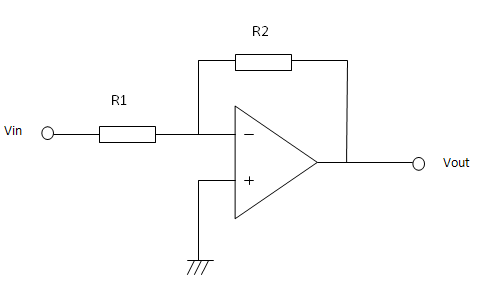
\includegraphics[width=0.6\linewidth]{Figures/inverseur.png}
	}
	\caption{Étage inverseur utilisé dans l'adaptation de tension.}
	\label{fig:inverseur}
\end{figure}

La fonction de transfert de cet étage d'amplification peut être calculée par l'équation \ref{eq:inverseur}. Ainsi, on fixe respectivement les valeurs des résistances $R1$ et $R2$ à $11Kohm$ et $3.3Kohm$.

\begin{align}\label{eq:inverseur}
   Vout = -Vin \times ( \frac{R2}{R1} )
\end{align}

Cet étage permet théoriquement d'amener la tension entre $-5V$ et $+5V$ à une tension comprise entre $-1.5V$ et $+1.5V$. En pratique, à cause des variations de valeurs des composants, et des caractéristiques de l'amplificateur opérationnel utilisé (imperfections statiques, tension d'offset), la tension est ramenée entre $-1.75V$ et $1.5V$.

Le deuxième étage est un offset réalisé par un montage sommateur inverseur permettant de repasser la plage de tension dans un intervalle positif. Le montage est décrit par la figure \ref{fig:sommateur1}. 

\begin{figure}
	\centering
	\fbox{
		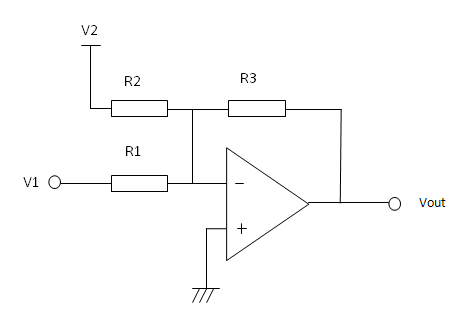
\includegraphics[width=0.6\linewidth]{Figures/sommateur.png}
	}
	\caption{Étage sommateur utilisé dans l'adaptation de tension.}
	\label{fig:sommateur1}
\end{figure}

La fonction de transfert de cet étage d'amplification peut être calculée par l'équation \ref{eq:sommateur1}. 

\begin{align}\label{eq:sommateur1}
   Vout = -R3 \times ( \frac{V1}{R1} + \frac{V2}{R2})
\end{align}

Soit, si $R1 = R2 = R3$ : 

\begin{align}\label{eq:sommateur2}
   Vout = -(V1 + V2)
\end{align}

Ainsi, V1 représente la sortie du premier étage d'amplification et V2 la tension d'offset à ajouter à V1 pour faire passer toute la plage de tension dans les tension négatives (en théorie donc -1.5V). Enfin le facteur $-1$ généré par la partie inverseuse du montage permet de repasser l'intervalle de tension dans les tensions positives uniquement.

Le plus important pour le signal final est de ne pas dépasser $3.3V$ pour les crêtes hautes et de ne pas passer sous les $0V$ pour les crêtes basses. Le signal doit également être centré par rapport à cette plage de tension, et donc être centré aux alentours de $1.75V$.

La figure \ref{fig:adapttension} présente le schéma électronique utilisé sur chaque canal EMG avant de le connecter au PIC32.

\begin{figure}
	\centering
	\fbox{
		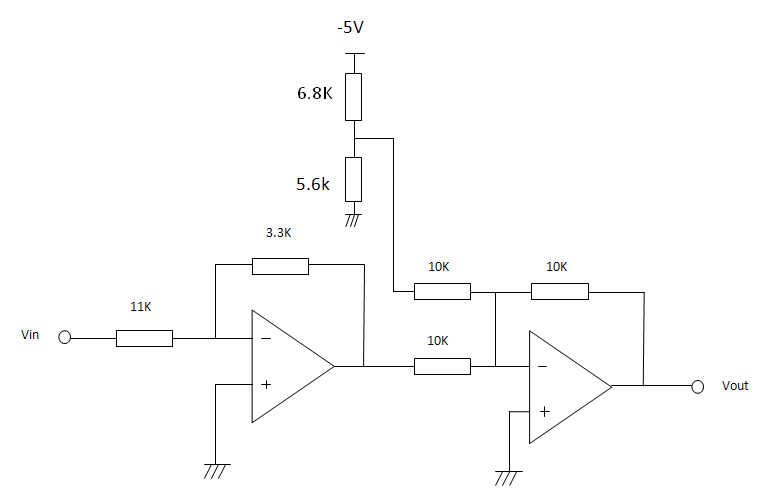
\includegraphics[width=0.6\linewidth]{Figures/circuitadapt.png}
	}
	\caption{Circuit électronique d'adaptation de la tension de sortie des électrodes.}
	\label{fig:adapttension}
\end{figure}

Cependant il est à souligner que la valeur exacte des composants électroniques varie suivant leur tolérance (5\% pour les composants utilisés ici). Ainsi le voltage correspondant au 0 peut ainsi varier (1.72V, 1.68V, …) et un offset sera donc présent sur les valeurs enregistrées par le convertisseur du PIC. 

Le schéma \ref{fig:adapttension} présente les valeurs de composants pratiques pour la réalisation du circuit. Celles-ci sont définies en tenant compte des imperfections statiques des amplificateurs et des variations des composants.


\subsection{Liaison à l'Ordinateur}

Une fois les électrodes connectée au microcontrôleur, celui-ci doit maintenant être connecté à l'ordinateur. Cette partie a pour but de présenter la liaison série réalisée entre la carte électronique du PIC32 et l'ordinateur utilisé pour visualiser les signaux en temps réel.

Dans un premier temps, les niveaux de tension du signal série délivré par le PIC32 ne sont pas compatibles avec ceux utilisés et transmis par l'ordinateur. En effet, le PIC fournit un signal entre 0V et +3.3V alors que les signaux du port série d'un ordinateur sont compris entre +12V et -12V. 

Afin de faire la transition entre ces deux niveaux de tension, un composant électronique intégré est utilisé : un MAX3232, présenté sur la figure \ref{fig:max3232}.

\begin{figure}
	\centering
	\fbox{
		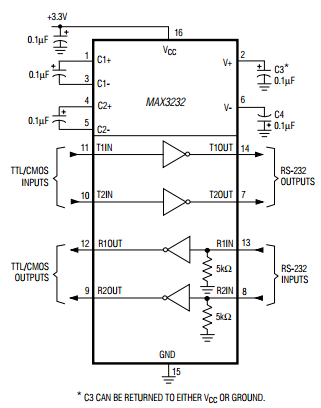
\includegraphics[width=0.6\linewidth]{Figures/max3232.png}
	}
	\caption{Circuit de câblage type du composant max3232, extrait de la documentation officielle du composant produit par \cite{MAXIM3232}.}
	\label{fig:max3232}
\end{figure}

Une fois la liaison physique réalisée, un protocole de transmission de données a été mis en place. En effet, les données arrivant sur le port série en RS-232 étant traitées octet par octet, il a fallu mettre en place une trame de données afin que celles-ci soit réceptionnées correctement, et permettant de vérifier que toutes les données reçues sont bien intègres.
Le début de trame (SOF, Start of Frame) est constitué de 4 octets fixes, ne changeant jamais de valeur. Ceci constitue une protection contre une mauvaise détection de début de trame. En effet, la même séquence de quatre octets est très improbable de se présenter en tant que données, et de ce fait on aura peu de chance de détecter un mauvais début de trame. Viennent ensuite les données. La longueur en octets des données à transmettre sur la liaison série est facilement configurable et modifiable à la fois dans le programme du PIC32 et dans le programme de l'application de monitorage sur l'ordinateur.
Ensuite, les deux octets suivants concernent le contrôle de redondance cyclique (CRC) qui permet de vérifier que la trame reçue n'a pas perdu d'information, ou n'a pas vu un de ses octets corrompu lors du transfert. Le CRC est une valeur sur 2 octets obtenue grâce à un calcul récursif simple dont l'opération mathématique principale est une division modulo 2 dont le reste est le CRC. %TODO : detailler CRC

Le CRC est calculé en prenant pour entrée uniquement la partie données de la trame. A la réception d'une nouvelle trame, le CRC des données est calculé, puis comparé au CRC transmis dans la trame. Si les deux CRC sont identiques, c'est que la trame est intègre, sinon, la trame est considérée comme non valide, et les données ne sont pas enregistrées, car corrompues.

Enfin, la fin de trame (EOF, End of Frame), est composé de 2 octets fixes qui ne changent pas non plus de valeur afin de détecter quand une fin de trame est réceptionnée. La figure \ref{fig:serialframe} présente le schéma global de la trame utilisée dans le cadre de la liaison série.

\begin{figure}
	\centering
	\fbox{
		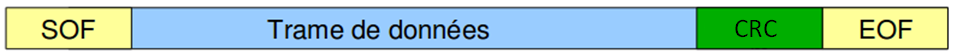
\includegraphics[width=\linewidth]{Figures/serialframe.png}
	}
	\caption{Format de la trame utilisée dans le cadre de la liaison série.}
	\label{fig:serialframe}
\end{figure}

Cette trame est utilisée autant dans les données allant du PIC32 vers l'ordinateur que pour les commandes de calibration envoyée au PIC32 par l'ordinateur.

\subsection{Liaison à Jaco}

Le fonctionnement interne de Jaco utilise un bus de type CAN comme mentionné dans le paragraphe \ref{ch:microcon}. Le bus CAN est un protocole de communication très répandu dans l'industrie et popularisé à l'origine par le secteur automobile. 

C'est un bus série opérant en mode différentiel, c'est à dire que deux fils transportent le même signal de manière complémentaire, permettant un contrôle de l'intégrité des données. Ce bus comprend également une couche protocolaire définissant des types de messages à envoyer à une adresse sur le bus. 

Dans un premier temps, il était impossible d'implanter directement le prototype du système directement dans le bras Jaco, ou même d'y faire rentrer des câbles pour s'y connecter. 

Kinova livre avec le bras robotique des librairies de programmation permettant à un programme fait par un utilisateur de se connecter à Jaco et de lui envoyer des commandes ou des fichiers de configuration. 

Le système au stade de prototype étant connecté un ordinateur par une liaison série, il est aisé de se servir de l'ordinateur comme intermédiaire entre le système de détection de mouvement et le bras Jaco lui-même.

De ce fait, le programme de monitorage des données du système doit également s'interfacer avec Jaco de manière à lui transférer des commandes en fonction des mouvements détectés. Cette connexion est effectuée grâce à la liaison USB disponible sur Jaco et utilise les librairies de programmation fournies par Kinova.

\subsection{Schéma matériel Global}

La partie \ref{CHarchimat} présente les différentes composantes nécessaire à la réalisation matérielle du projet. Cette partie a pour but de synthétiser tous les choix effectuer de manière à donner du recul et un point de vue global du prototype entier. 

Détaillons dans un premier temps les entrées et sorties du PIC32. 

Contrairement à beaucoup d'autres microcontrôleurs plus petits, le PIC32 ne possède pas d'entrées/sorties qui soit re-localisables. C'est à dire que l'on n'est pas en mesure de choisir quel périphérique prend ses entrées et sorties sur des pattes spécifiques du composants. Ceci implique donc des contraintes de câblage pour relier les électrodes et la liaison série sur celui-ci. 

Ainsi on voit sur la figure \ref{fig:cablagePic} que les quatre électrodes sont reliées via l'adaptation de tension au entrées anaologiques AN1, AN2, AN3 et AN4 du PIC32. 

\begin{figure}
	\centering
	\fbox{
		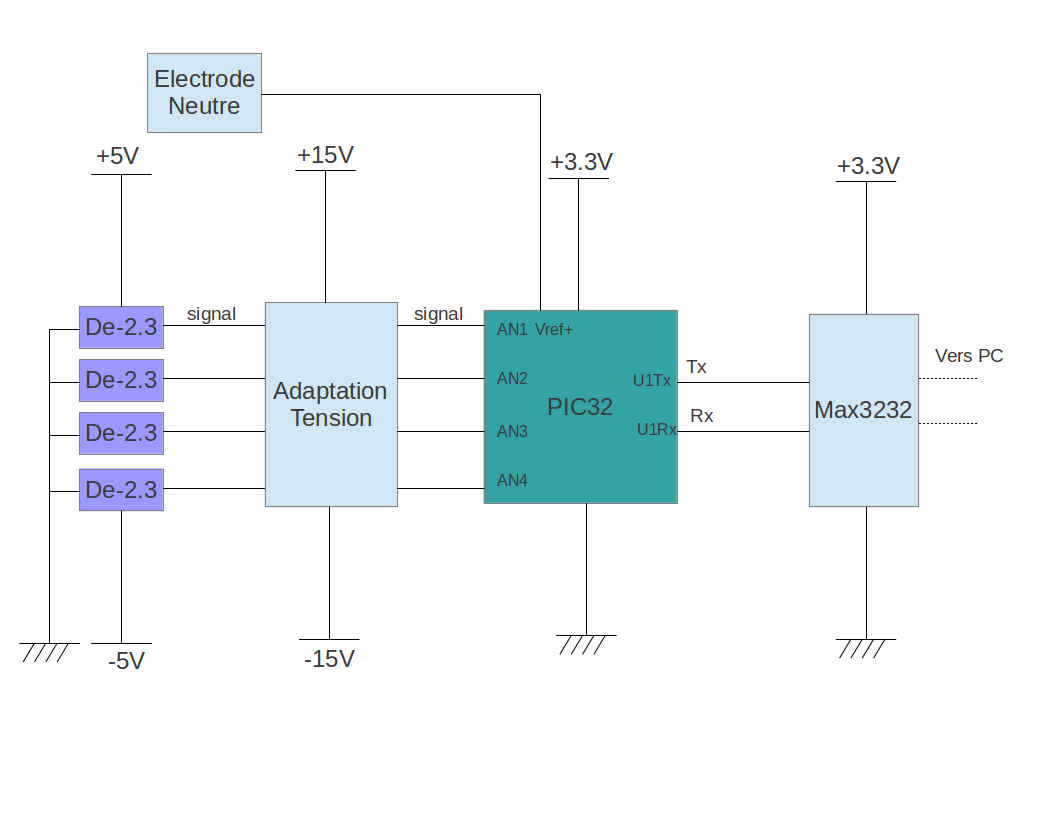
\includegraphics[width=\linewidth]{Figures/cablagePic.png}
	}
	\caption{Schéma bloc présentant le câblage de la partie électronique du projet}
	\label{fig:cablagePic}
\end{figure}

L'électrode neutre est reliée au PIC par l'entrée VRef+ qui sert de référence de mesure pour le convertisseur analogique/numérique du microcontrôleur. 

Une UART (Universal asynchronous receiver transmitter) du PIC32 est utilisée pour réaliser la liaison série à l'ordinateur. Les deux lignes de transmission et réception Tx et Rx sont reliées au Max3232 qui adapte les tensions entre le PIC et l'ordinateur par les entrées sorties U1Tx et U1Rx (UART 1 Tx et UART 1 Rx).

Si l'on prend maintenant un point de vue plus haut, nous sommes en mesure d'étudier le système dans son ensemble comme le présente la figure \ref{fig:archiMatTot}.

\begin{figure}
	\centering
	\fbox{
		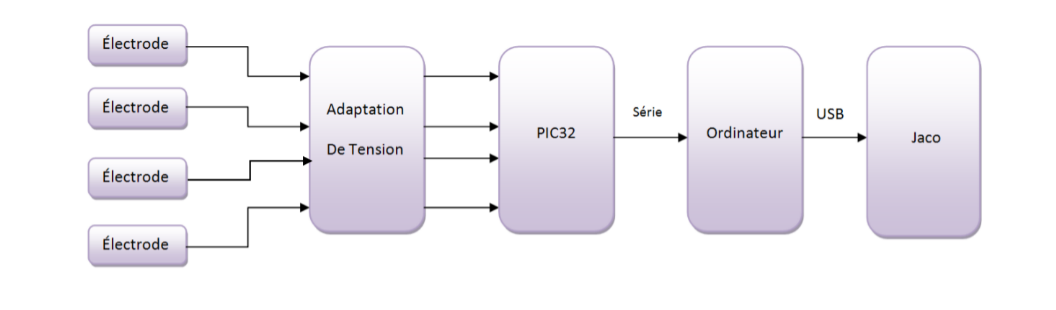
\includegraphics[width=\linewidth]{Figures/archiMatTot.png}
	}
	\caption{Schéma bloc présentant le système global}
	\label{fig:archiMatTot}
\end{figure}

Il est nécessaire de préciser que dans cette architecture, l'ordinateur ne sert que d'intermédiaire entre le microcontrôleur et Jaco. En effet, le microcontrôleur effectue la totalité des calculs. Le mouvement effectué par l'utilisateur est envoyé sur la liaison série à l'ordinateur qui transmet la commande choisie à Jaco via la liaison USB. 

Il est également à noter que cette architecture va induire un délai de traitement impossible à quantifier précisément. En effet, l'ordinateur n'étant pas temps réel au sens strict, le temps entre l'information d'un mouvement effectué et le nouvement de Jaco (ou toute autre action) commandé par USB est imprévisible précisément et sera beaucoup plus long que si le PIC32 était relié à Jaco directement par un bus CAN. 

Ainsi, les temps de traitement mesurés caractériseront uniquement la partie calculatoire effectuée sur le PIC32, et non le temps entre le signal perçu par l'électrode et la commande appliquée sur le bras robotique.

\section{Choix des Caractéristiques du Signal à utiliser et des Outils algorithmiques et Mathématiques}

Une fois les choix matériel effectués et le calculateur choisi, l'étape de réalisation suivante est le choix des calculs a effectuer pour le bon fonctionnement de la détection d'activité musculaire. 

Cette partie se décomposera en plusieurs sous partie à des fin de compréhension. La première partie concernera la manière de découper les fenêtre d'échantillons du signal EMG. 

La seconde partie concernera le coeur du projet : la détection d'activité musculaire et les outils mathématiques utilisés pour la réaliser. Dans un premier temps, l'utilisation de l'énergie de Teager-Keiser sera détaillée puis l'utilisation d'un vote à la majorité pour le lissage de la détection sera expliquée et enfin la calibration de la détection.

Enfin une dernière partie détaillera le choix du filtre numérique appliqué sur le signal et la manière dont celui-ci est calibré pour chaque sujet et chaque canal EMG.

\subsection{Découpage des fenêtres d'échantillons}

Comme vu dans la revue de littérature, l'exploitation du signal EMG ne se fait pas échantillon par échantillon, le signal est découpé en fenêtre puis chaque fenêtre est utilisée pour calculer des caractéristiques. Ces caractéristiques sont utilisées dans un classificateur pour déterminer le mouvement effectué par l'utilisateur. 

La taille de la fenêtre influe principalement sur les performances du classificateur, car une petite fenêtre induit un biais en raison de la variance du signal qui peut entraîner une classification fausse. 

Le projet s'étant affranchi du classificateur, s'affranchit également du problème de fenêtrage du signal, dans le sens ou son choix ne joue que sur le temps de traitement de celui-ci, en effet, plus une fenêtre est longue plus le temps de calcul pour la traiter est long. 

Toute fois, plus une fenêtre est courte, plus le délai avant de recevoir la prochaine fenêtre est également court. 

Le choix du découpage en fenêtre du signal est donc ouvert et peut être fait en prenant tous les critères algorithmiques restant, à savoir le fonctionnement interne du PIC32, et des librairies qu'il met à disposition. 

En effet, comme la partie \ref{CHfiltrage} le présentera, le PIC32 met à disposition une librairie flottante incluant une fonction effectuant le calcul d'une transformée de Fourrier rapide (Fast Fourrier Transfor - FFT). Ces fonctions sont nécessaires au filtrage appliqué sur le signal. Les fonctions de cette librairie étant spécialement prévues pour l'architecture du PIC32, celles-ci ont une vitesse d'exécution optimale. La fonction FFT fournie par la librairie PIC32 est disponible sous 3 formes : 

\begin{itemize}
 \item fft8
 \item fft16
 \item fft32
\end{itemize}

Le nombre mentionné dans chaque fonction correspond au nombre d'échantillons dans le signal sur lequel la fft sera calculée. Ainsi fft8 prend en paramètre une fenêtre de signal de 8 échantillons et renvoie une FFT sur 8 points.

En conclusion, trois tailles de fenêtrage sont ici possibles de manière à faciliter le traitement du signal : 8, 16 et 32 échantillons. D'autres fenêtres seraient possible, mais il faudrait alors les découper en sous-fenêtres afin de pouvoir les filtrer. 

\subsection{Détection d'activité musculaire}\label{CHdetect}

La détection d'activité musculaire est le coeur du projet de contrôle de Jaco par EMG. En effet, le fait de s'être affranchi d'un classificateur implique que cette étape se déroule de manière optimale et toujours cohérente.

Une première partie présentera la caractéristique principale utilisée pour détecter les activités musculaires : l'énergie de Teager-Keiser (TKE). 

Puis dans un second temps, le système de vote à la majorité sera détaillé. En effet, fixer un simple seuil sur le TKE du signal entraine une détection d'activité en changement d'état permanent, parfois à chaque nouvelle fenêtre. Le vote à la majorité permet de lisser cette détection de manière à obtenir une détection d'activité continue sous la forme d'un échelon.

Enfin, le système de calibration pour chaque muscle et chaque sujet sera présenté.

\subsubsection{Énergie de Teager-Keiser}
%TODO faire des tests sur la valeur absolue du tke pour voir si ca marche toujours. faire plein de screen shots a foutre la dedans.

L'étude de \cite{li2007} a montré qu'une caractéristique du signal EMG est très efficace pour la détection d'activité musculaire automatique : l'énergie de Teager-Keiser (TKE). Cette caractéristique s'apparente à un taux de variation simple du signal en comparant un échantillon à son précédent et à son suivant. Le TKE se calcule comme présenté par l'équation \ref{eq:tke}.

\begin{align}\label{eq:tke}
   TKE(k) = x^2(k) - x(k-1)*x(k+1) 
\end{align}

Ainsi, une fois une fenêtre acquise complètement, le TKE instantané (sur chaque échantillon) est calculé. La figure \ref{fig:tkeinstant} montre le TKE instantané obtenu sur un signal EMG donné.

\begin{figure}
	\centering
	\fbox{
		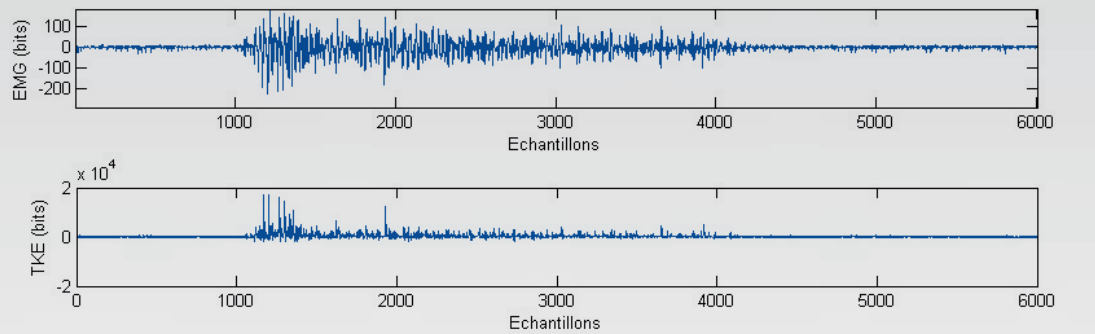
\includegraphics[width=0.8\linewidth]{Figures/tkeinstant.png}
	}
	\caption{TKE instantané calculé sur un signal EMG}
	\label{fig:tkeinstant}
\end{figure}

Cependant, ce TKE par échantillon est difficile à utiliser directement, car il est très variable et fixer un seuil efficace pour détecter les activités serait très compliqué. Pour faciliter son exploitation, on effectue la moyenne du TKE sur toute la fenêtre, afin d'en obtenir son enveloppe. De cette manière, un seuil de détection est applicable plus facilement. La figure \ref{fig:tkemoy} présente le passage du TKE instantané au TKE moyen.

\begin{figure}
	\centering
	\fbox{
		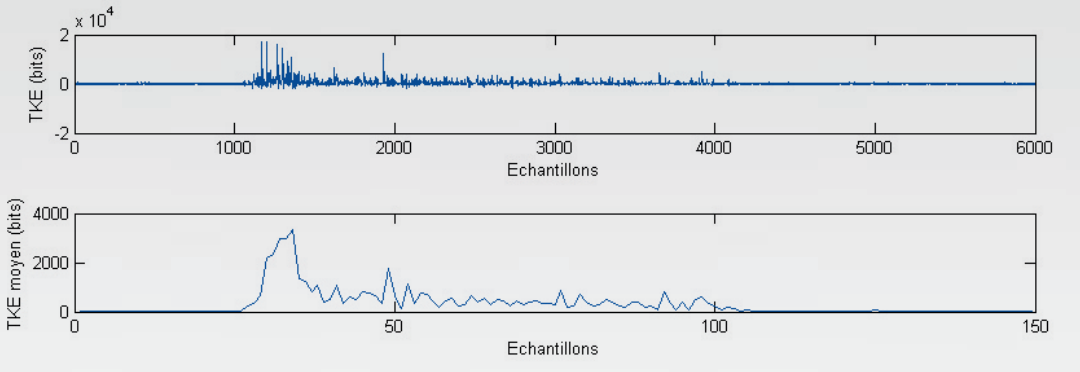
\includegraphics[width=0.8\linewidth]{Figures/tkemoy.png}
	}
	\caption{TKE moyen calculé sur un signal EMG}
	\label{fig:tkemoy}
\end{figure}

Une fois le TKE d'une fenêtre calculé, le but est de savoir si le muscle est activé ou non. Pour ce faire, un seuil doit être défini. Si le TKE de la fenêtre dépasse ce seuil, alors le muscle est considéré comme étant en activité.

\subsubsection{Calibrage du seuil de détection}

Une fois le système de détection d'activité musculaire défini, celui-ci doit ensuite être adapté à chaque utilisateur, et même à chaque muscle de cet utilisateur. En effet, chaque personne développe une force différente, de la même manière que chaque personne ne présente pas le même tonus musculaire lorsqu'il est au repos. 

Par exemple une personne stressée sera beaucoup plus contractée au niveau des trapèzes qu'une personne complètement détendue, et ce même sans avoir l'impression d'être contractée.

De manière à calibrer efficacement le seuil de détection d'activité musculaire, il nous faut récolter deux information pour chaque muscle : 

\begin{itemize}
 \item le tonus musculaire au repos
 \item le tonus musculaire en contraction isométrique maximum
\end{itemize}

On acquiert ces données en se basant sur le TKE d'un muscule lorsqu'il est au repos, ainsi que lorsqu'il est en contraction isométrique maximum, c'est à dire que le muscle se contracte au maximum, tout en maintenant l'articulation fixe. Les équations \ref{eq:calibZero} et \ref{eq:calibMax} présentent les calculs permettant d'obtenir les données.

\begin{align}\label{eq:calibZero}
   Tonus_{repos} = \frac{\sum_{n=1}^{20}TKE(x_{repos}(n))}{20} 
\end{align}

\begin{align}\label{eq:calibMax}
   Tonus_{max} = \frac{\sum_{n=1}^{20}TKE_{max}(x_{max}(n))}{20} 
\end{align}

où $x(n)$ représente une fenêtre de 16 échantillons du signal brut. On calcule donc la moyenne des TKE sur 20 fenêtres, ce qui correspond à une durée de $160ms$. 

Ainsi, l'utilisateur reste au repos, ou bien rentre en contraction maximum, on actionne alors la calibration grâce à l'interface graphique sur l'ordinateur pour enregistrer les tonus de chaque muscle.

Une fois les tonus musculaires recueillis, on sait maintenant qu'à chaque mouvement, l'utilisateur produira un signal EMG dont le TKE moyen sera entre son tonus de repos et son tonus maximum. 

Toutefois, il est peu probable que le tonus maximum soit atteint pendant un mouvement. En effet, une contraction isométrique produit un signal beaucoup plus gros qu'une contraction dans un mouvement lent. Le seuil de détection devra donc se trouver entre les deux tonus, le plus proche possible du tonus de repos sans qu'un bruit occasionnellement plus élevé sur le canal ne puisse passer au dessus du seuil. 

Le seuil a donc été fixé de manière heuristique à $1/4$ de l'intervalle entre le tonus de repos et le tonus maximum. La figure \ref{fig:seuilDetection} met en image la manière dont le seuil est fixé pour chaque muscle.

\begin{figure}
	\centering
	\fbox{
		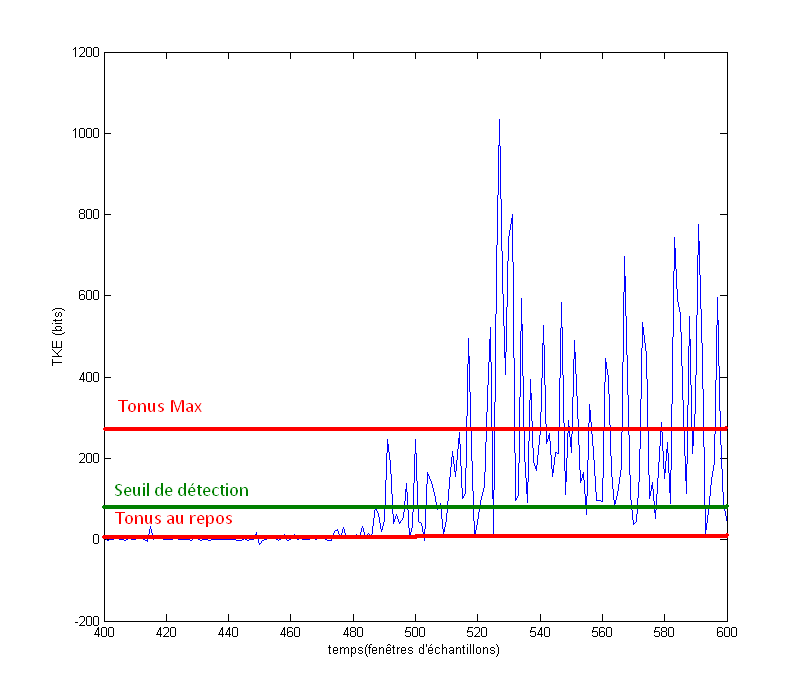
\includegraphics[width=0.6\linewidth]{Figures/tkeSeuil2.png}
	}
	\caption{Définition du seuil de détection d'activité musculaire pour un canal EMG}
	\label{fig:seuilDetection}
\end{figure}

\subsubsection{Vote à la majorité}

Le seuil fixé sur le TKE pour la détection d'activité permet donc de déterminer lorsqu'un muscle est en activité ou non, en observant lorsque ce seuil est dépassé. Cependant, le TKE variant au cours d'un mouvement, il se peut que celui-ci repasse par des moments proches de 0, même pendant un mouvement.

Ceci entraine alors une détection d'activité qui change alors souvent d'état comme le montre la figure \ref{fig:onsetSansVote}.

\begin{figure}
	\centering
	\fbox{
		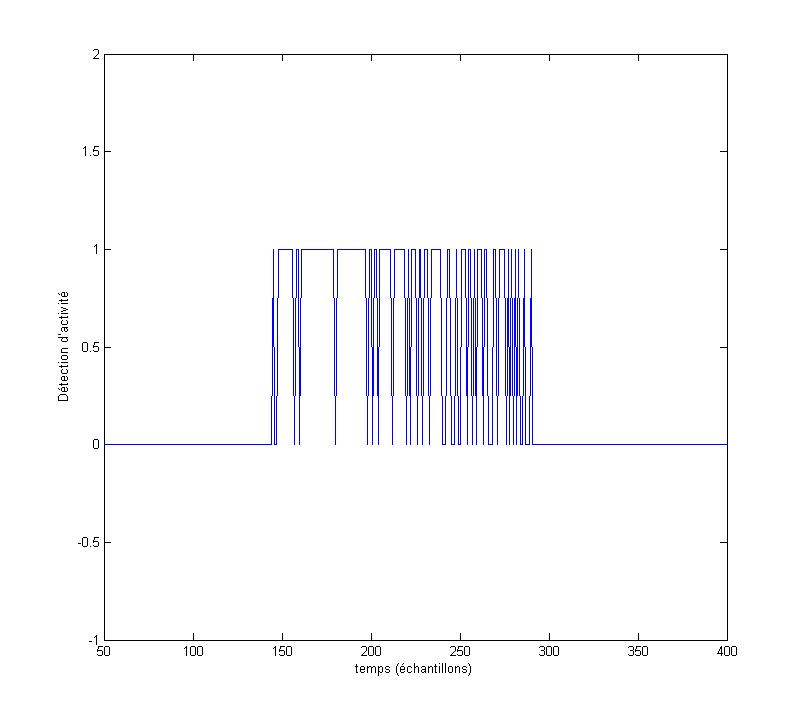
\includegraphics[width=0.42\linewidth]{Figures/onsetSansVote.png}
	}
	\caption{Détection d'activité musculaire brute, sans vote à la majorité.}
	\label{fig:onsetSansVote}
\end{figure}

Une conséquence supplémentaire est que si le seuil se veut d'être le plus bas possible afin d'augmenter la sensibilité du système, plus il est bas, plus le système est susceptible de détecter des faux positifs. 

Le choix du seuil de détection est donc difficile, voir impossible à choisir idéalement. En effet, un seuil trop haut ne sera plus assez sensible pour détecter des mouvements faibles et en ratera une parte, tandis qu'un seuil trop bas sera sensible mais détectera des faux positifs si le bruit sur le TKE le dépasse.

Afin de remédier à ces deux problèmes, une méthode inspirée du vote à la majorité de \cite{Chang1996} a été mise en place. La méthode mise en place par \cite{Chang1996} consiste à comparer la caractéristique d'une fenêtre au seuil. Puis, pour déterminer la détection d'activité, on effectue un vote à la majorité sur les cinq dernières fenêtres. Si la majorité des fenêtre est au dessus du seuil, l'activité musculaire est mise à 1, sinon elle est mise à 0.

Ce système permet d'éliminer la plupart des faux positifs. Toute fois, un inconvénient persiste. En effet, une fenêtre d'activation suffit à faire la différence entre une activité ou un repos. Ainsi, la détection d'activité peut toujours osciller entre 0 et 1, si la comparaison au seuil est différente à chaque nouvelle fenêtre, résultant en une activité en dents de scie comme sur la figure \ref{fig:onsetSansVote}.

La méthode mise au point pour le système consiste à mettre deux seuils de majorité et de minorité séparés. Ainsi, sur 32 fenêtres d'échantillons, si 16 ou plus sont au dessus du seuil de TKE, l'activité musculaire est mise à 1, puis, pour que celle-ci retombe à 0, il faut que le nombre de fenêtres au dessus du seuil retombe en dessous de 10. Cela permet de ne pas faire des allers-retours entre 15 et 16 fenêtres activées, qui entrainent des discontinuités de détection.

Le résultat de ce système de vote à la majorité est présenté par la figure \ref{fig:onsetAvecVote}.

\begin{figure}
	\centering
	\fbox{
		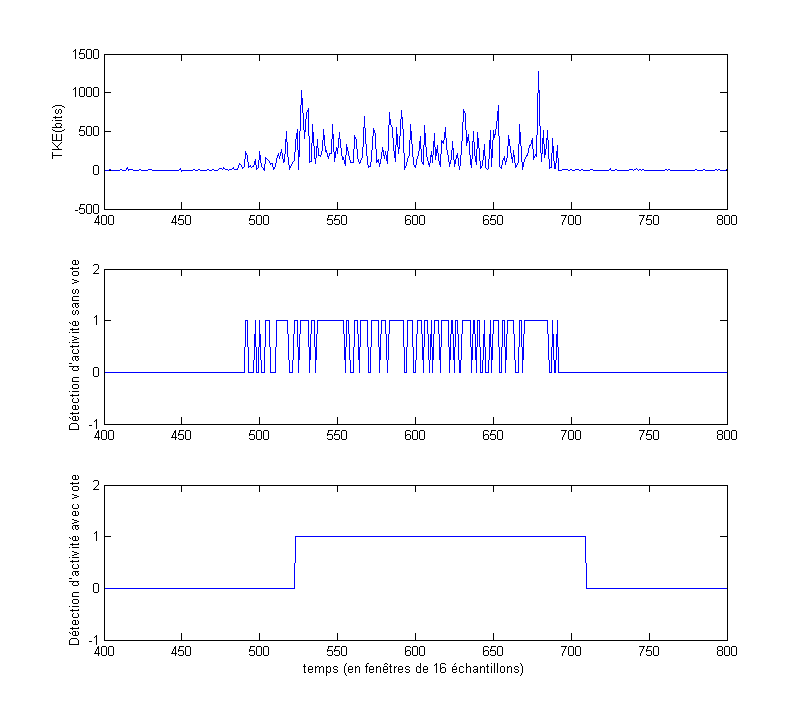
\includegraphics[width=0.6\linewidth]{Figures/onsetAvecVote.png}
	}
	\caption{Détection d'activité musculaire avec vote à la majorité.}
	\label{fig:onsetAvecVote}
\end{figure}

On observe qu'il n'y a plus de retour à 0 de la détection d'activité, et les faux positifs occasionnels ont également été retirés. Ce vote à la majorité provoque toute fois une légère latence de détection, en effet, il faut attendre que 16 fenêtres sur 32 soient au dessus du seuil de détection pour que l'activité soit détectée.

\subsection{Filtrage}\label{CHfiltrage}

Dans un premier temps, le système a été réalisé sans filtrage numérique. Ainsi le système fonctionnait uniquement en se basant sur la détection d'activité musculaire décrite au chapitre \ref{CHdetect}.

Les tests ont été concluants concernant la détection d'activité seule. Cependant le système a présenté une faiblesse : pour être détecté, un mouvement doit être très ample et comporter une composante isométrique. Les mouvements simples et lents ne demandant pas beaucoup de force ne sont pas détectés par le système. 

En résumé, le système manque de précision, et son utilisation chez des personnes blessées médullaires ayant potentiellement moins de tonus musculaire qu'une personne en bonne santé est alors compromise. 

Une solution est de filtrer le signal EMG brut de manière à amplifier les phases d'activité musculaire et diminuer au maximum le bruit de mesure. 

L'utilisation d'un filtre prédictif est donc préconisée pour effectuer ce travail. 

Cette partie présente le filtre prédictif mis en place dans le système dans le but d'augmenter sa sensibilité tout en diminuant le bruit de mesure. Une brève description du filtre sera d'abord effectuée, puis le calibrage de celui-ci sera décrit dans une seconde partie, pour enfin terminer par la description détaillée du filtre et de son algorithme.

\subsubsection{Concept}

Le but du filtrage prédictif est de pouvoir prédire quelles partie du signal le filtre doit amplifier, et quelles parties de ce même signal il doit écraser.

Dans notre cas, la partie du signal à écraser est le bruit analogique mesuré par les ADC du PIC32, tandis que la partie du signal à amplifier est le signal EMG généré par le muscle sur lequel est collée l'électrode.

Le filtre ayant deux élément à reconnaitre (le bruit et le signal), il faut en caractériser un des deux, et définir que lorsque l'on ne le détecte pas, c'est que l'on est en présence de l'autre. Ainsi, on choisit de caractériser le bruit. Lorsque le système détecte la présence du bruit, alors le signal est écrasé, lorsqu'il ne le détecte pas, c'est qu'un EMG est présent dans le signal, il est alors amplifié.

Pour caractériser le bruit, on utilise les caractéristiques fréquentielles du signal. Le but est donc d'isoler le spectre d'amplitude du bruit afin d'en faire un modèle de comparaison. On enregistre un signal sans EMG et on calcule le spectre d'amplitude moyen de ce signal. C'est la bande de base.

Puis à chaque nouvelle fenêtre, on compare le spectre d'amplitude de cette fenêtre à celui de la bande de base pour calculer une probabilité de présence du bruit. Cette probabilité permet de fixer un gain qui amplifiera ou écrasera le spectre d'amplitude et donc par extension, le signal.

Il est également à noter que l'on ne veut pas créer de déphasage du signal. La phase du signal sera donc isolée de la fft pour être réutilisée sans modification pour reconstruire le signal après que le spectre d'amplitude a été transformé.  

\subsubsection{Calibrage du Filtre}

Une fois le concept du filtre posé, le mode de fonctionnement précis du filtre va maintenant être détaillé. La première étape de la réalisation du filtre est son calibrage, ou l'enregistrement de la bande de base. 

Le calibrage du filtre s'effectue sur une partie de signal où l'on est sur qu'aucun EMG ne sera présent. On demande donc à l'utilisateur de ne pas bouger pendant l'acquisition de la bande de base. 

Le signal est alors acquis par fenêtre. Lorsqu'une fenêtre est acquise, on la normalise, c'est à dire qu'on retire sa moyenne à chaque échantillon (eq:normalCalib où $NFFT$ = 16), puis on calcule sa FFT (équation \ref{eq:fftcalib}).

\begin{align}\label{eq:normalCalib}
   x_{k=1}^{k=NFFT}(k) = x(k) - \frac{\sum_{n=1}^{NFFT}x(n)}{NFFT}
\end{align}

\begin{align}\label{eq:fftcalib}
   fft = FFT_{16}(x(k)) 
\end{align}

La $fft$ calculée par cette opération est donc un tableau de 16 nombres complexes représentant la transformée de fourrier de la fenêtre.

Une fois cette FFT calculée, on met la phase du signal de côté pour ne garder que le spectre d'amplitude $M$ de la fenêtre (équation \ref{eq:amplCalib}).

\begin{align}\label{eq:amplCalib}
   M_{k=1}^{k=NFFT}(k) = \Vert fft(k) \Vert^2 
\end{align}

On garde ensuite en mémoire ce spectre d'amplitude, puis on répète l'opération sur 20 fenêtres. Une fois les 20 spectres d'amplitude acquis, on calcule le spectre d'amplitude moyen de ces 20 fenêtres (équation \ref{eq:ampMoyCalib}).

\begin{align}\label{eq:ampMoyCalib}
   BandeBase = \frac{\sum_{n=1}^{20}amplitude(n)}{20}
\end{align}

Ce spectre d'amplitude moyen constitue la bande de base qui sera comparée à chaque fenêtre du signal pour déterminer à chaque fenêtre la probabilité de présence du bruit dans le signal.

\subsubsection{Description du Filtre}

Une fois la bande de base du filtre calibrée, le filtre peut être mis en fonctionnement à chaque fenêtre de signal acquise. Cette partie détaille le fonctionnement algorithmique du filtre. 

Une nouvelle fenêtre est acquise. Dans un premier temps, elle est sujette au même traitement que pour la calibration : elle est normalisée (équation \ref{eq:normalCalib}) puis sa FFT est calculée (équation \ref{eq:fftcalib}).

Une fois la FFT obtenue, on sépare le spectre d'amplitude (équation \ref{eq:amplCalib}) de la phase $\phi$ qui cette fois-ci est aussi calculée (équation \ref{eq:phaseFiltre}). En effet, celle-ci sera nécessaire pour reconstruire le signal une fois que l'amplitude aura été modifiée.

\begin{align}\label{eq:phaseFiltre}
   \phi(k) = atan2(\Im(fft(k)), \Re(fft(k)))
\end{align}

On calcule ensuite la probabilité a posteriori $postsnr$ de présence du filtre en faisant le rapport entre le spectre d'amplitude de la fenêtre et le spectre d'amplitude moyen (équation \ref{eq:probFiltre}).

\begin{align}\label{eq:probFiltre}
   postsnr(k) = \frac{M(k)}{M_{Bande de base}} - 1
\end{align}

Cette probabilité est ensuite limitée pour ne pas créer de distorsion provoquée par une valeur trop petite (équation \ref{eq:maxPostsnr}).

\begin{align}\label{eq:maxPostsnr}
   postsnr(k) = \max(postsnr(k), 0.01)
\end{align}

On compare ensuite la probabilité obtenue avec la celle obtenue avec le spectre d'amplitude de la fenêtre précédente. Cette méthode est appelée méthode de la "décision adaptative" (équation \ref{eq:etaFiltre}). Une nouvelle amplitude est alors calculée en appliquant cette probabilité sur l'amplitude d'origine (équation \ref{eq:newMagEta}).

\begin{align}\label{eq:etaFiltre}
   eta(k) = \alpha * \frac{M(k-1)}{M_{Bande de base}} + (1 - \alpha) * postsnr(k)
\end{align}

\begin{align}\label{eq:newMagEta}
   M_{new}(k) = \frac{eta}{eta+1} * M(k)
\end{align}

On calcule ensuite le gain à appliquer sur le spectre d'amplitude en comparant l'amplitude sur laquelle on a appliqué les probabilités a priori avec le spectre d'amplitude moyen (équation \ref{eq:tsnr1}, \ref{eq:tsnr2}, \ref{eq:Gtnsr} et \ref{eq:Gtsnr2}).

 \begin{align}\label{eq:tsnr1}
   tsnr(k) = \frac{M_{new}(k)}{M_{Bande de base}}
\end{align}

 \begin{align}\label{eq:tsnr2}
   Gtsnr(k) = \frac{tsnr(k)}{tsnr(k)+1}
\end{align}

 \begin{align}\label{eq:Gtnsr}
   Gtsnr(k) = \max(Gtsnr(k), 0.01)
\end{align}

\begin{align}\label{eq:Gtsnr2}
   M_{new}(k) = Gtsnr * M(k)
\end{align}

Une fois la nouvelle amplitude calculée, il ne reste plus qu'à reconstruire la fft du signal, en réunissant l'amplitude et la phase (équation\ref{eq:reconFiltre1} et \ref{eq:reconFiltre2}).

\begin{align}\label{eq:reconFiltre1}
   \Re(fft(k)) = M_{new}(k) * cos(\phi(k))
\end{align}

\begin{align}\label{eq:reconFiltre2}
   \Im(fft(k)) = -M_{new}(k) * sin(\phi(k))
\end{align}

Une fois fait, on effectue la transformée de fourrier inverse pour retrouver le signal EMG filtré.

\section{Architecture Logicielle}

Les parties précédentes ont présenté l'architecture matérielle ainsi que les outils mathématiques utilisés dans le projet. La derniere grande partie technique à présenter restante est donc l'architecture logicielle. 

En effet, tout en prenant en compte les choix effectués dans la partie précédente, la manière de les réaliser et de les connecter ensembles doit être présentée. 

Ainsi, ce chapitre présentera d'abord le fonctionnement du firmware, c'est à dire le programme exécuté sur le PIC32 puis présentera le fonctionnement de l'application de monitorage des signaux, qui permet aussi la connexion du système au bras Jaco et qui est exécutée sur un ordinateur. 

\subsection{Firmware}

Le firmware est le nom donné à un programme tournant sur un microcontrôleur, ou sur une carte électronique. Ce firmware est un programme développé dans un langage dépendant du microcontrôleur choisi pour le projet. 

Le PIC32 est programmable en langage C, ainsi qu'en assembleur bien qu'il soit peu utilisé, excepté pour les parties de code nécessitant une grande optimisation. 

Cette partie décrira le fonctionnement du PIC32 ainsi que l'algorithme global du firmware. 

\subsubsection{Fonctionnement et Configuration Globale du PIC32}

Pour présenter le firmware, il est important de présenter la manière de fonctionner du PIC32. La différence principale entre un microcontrôleur et un ordinateur moderne est qu'il est impossible d'exécuter plusieurs programmes en parallèle sur un microcontrôleur. En effet, c'est le système d'exploitation qui permet dans un ordinateur de paralléliser les opérations effectuées. 

Ainsi, un microcontôleur n'effectue qu'une seule série d'opérations : celle de son programme. Un programme est une suite d'instructions élémentaires compilées dans un fichier binaire. Cette suite d'instruction est inscrite dans la mémoire de programme du microcontrôleur et chaque instruction possède une adresse dans cette mémoire. Le compteur de programme (PC - program counter) et un nombre contenant l'adresse mémoire de l'instruction en cours. Une fois que cette instruction est finie, le PC est incrémenté pour passer à l'instruction suivante et jusqu'à ce que le programme se termine. 

Cependant le microcontrôleur possède des périphériques dédiés capables d'effectuer les opérations pour lesquelles ils sont prévus sans influencer le déroulement du programme principal. Par exemple, le convertisseur analogique-numérique (ADC) enregistre les échantillons du signal sans que cela ait à figurer dans le programme. 

Ces périphériques possèdent des interruptions, qui permettent de signifier au programme lorsque des données sont accessibles. Ces interruptions sont déclenchées quand une condition est remplie et sont une fonction spécifique qui n'est exécutée que lorsque la condition est remplie. Par exemple, il est possible de configurer l'ADC du PIC32 pour qu'il déclenche une interruption à chaque fois qu'il a fini d'acquérir 16 samples. 

Lorsqu'une interruption est déclenchée par un périphérique, le déroulement du programme est arrêté. L'adresse de l'instruction où il s'est arrêté est mise en mémoire, puis le code de la fonction d'interruption est exécuté. Une fois que cette fonction est terminée, le programme reprend son cours normal à l'adresse qui avait préalablement été mise en mémoire. 

Ce système d'interruption permet d'effectuer automatiquement des opérations comme l'acquisition d'un signal, ou l'envoi et la réception de messages sur le port série sans influencer le programme principal, et donc gagner du temps de calcul. 

Cependant, les interruptions bloquent le cours normal du programme principal. Les interruptions doivent donc être le plus courtes possibles pour ne pas perdre trop de temps dedans. 

Il est donc important de bien choisir quels calculs sont effectués dans les interruptions, et quels calculs sont faits dans le programme principal. 

Une interruptions peut également être interrompue par une autre interruption. Un système de priorité détermine l'ordre dans lequel ces interruptions ont lieu. Une interruption ne pourra jamais interrompre une autre interruption ayant une priorité plus haute. Ainsi l'interruption encours se terminera avant que l'autre puisse s'effectuer. 

Ainsi, les deux périphériques utilisés dans le système fonctionneront à base d'interruptions, à savoir l'ADC permettant l'acquisition des quatre canaux, et l'UART permettant la communication série. 

L'ADC du PIC32 permet de scanner plusieurs entrées les unes après les autres. Ainsi il faut donc multiplier la fréquence d'échantillonnage par le nombre de canaux afin de pouvoir acquérir tous les canaux à la bonne fréquence. On fixe donc la fréquence d'échantillonnage à 8KHz pour que chaque canal soit échantillonné à 2KHz. 

L'interruption de l'ADC est configurée pour être déclenchée après avoir acquis le plus d'échantillons possible, soit 8 échantillons. Ainsi, tous les 8 échantillons, correspondant à 2 échantillons par canal, l'interruption de l'ADC est déclenchée. 

L'UART du PIC32 quant à elle possède deux interruptions, une pour l'envoi de données, et l'autre pour la réception. Ces interruptions sont déclenchées respectivement à l'envoi et à la réception d'un octet complet. Ainsi, à chaque octet reçu, celui-ci est mis en mémoire dans l'interruption, et à chaque octet envoyé, on met l'octet suivant dans le "buffer" d'envoi.

\subsubsection{Alogorithme global}

Une fois le fonctionnement global du PIC32 et de ses interruptions décrit, l'algorithme du programme principal ainsi que ceux des interruptions peuvent maintenant être présentés en détail. 

Nous nous intéressons dans un premier temps au fonctionnement du programme principal, puis les algorithmes des deux interruptions principales seront détaillés. 

Le programme principal du firmware commence par initialiser tous les périphériques du PIC32 qui seront utilisés, ainsi que l'horloge principale et les configurations des interruptions. C'est à ce moment que l'ADC et le port série sont configurés. 

Une fois les initialisations effectuées, le programme entre dans une boucle infinie qui constitue la colonne vertébrale du programme. Les actions réalisée par cette boucle sont présentées par la figure \ref{fig:mainloop}.

\begin{figure}
	\centering
	\fbox{
		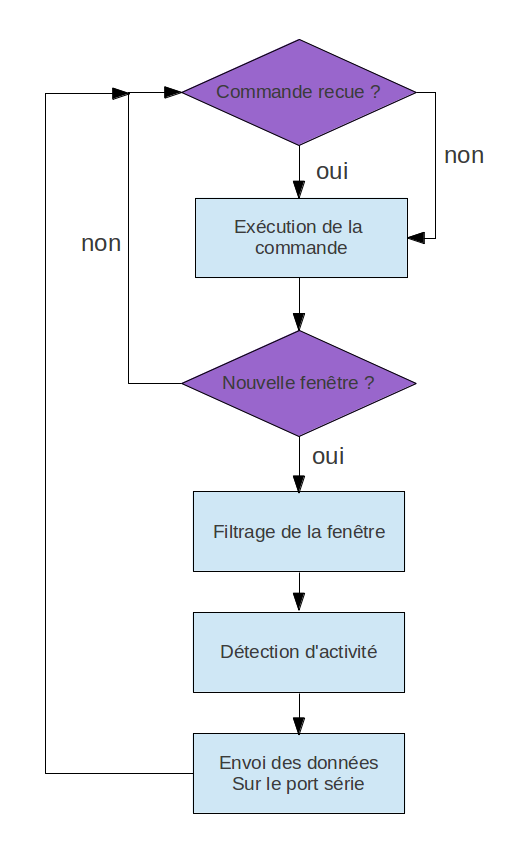
\includegraphics[width=0.6\linewidth]{Figures/mainloop.png}
	}
	\caption{Boucle inifinie du programme principal.}
	\label{fig:mainloop}
\end{figure}

La boucle commence ainsi par vérifier si une commande à été reçue sur le port série. Les commandes reçues sur le port série sont les commandes de calibration du système. Ainsi chaque commande est constituée du type de calibration a effectuer, c'est à dire une calibration du tonus maximum, une calibration du tonus au repos ou bien la calibration de la bande de base du filtre, et le numéro du canal sur lequel effectuer cette calibration. 

On vérifie ensuite si une fenêtre de signal a été acquise en entier. Si c'est le cas, cette fenêtre est filtrée, puis passée dans la fonction de détection d'activités. Enfin les données calculées sont envoyées sur le port série pour être monitorées.

Il est à noter que le filtrage n'est effectué que si la calibration de la bande de base a bien eu lieu précédemment, mais ce test n'est pas affiché sur le diagramme à des fins de clarté. 

Cette partie montre comment le signal est traité, présentons maintenant comment celui-ci est acquis. La figure \ref{fig:adc} présente la routine d'interruption de l'ADC du PIC32. Celle-ci est déclenchée à chaque fois que 8 échantillons ont été acquis en tout, soit 2 échantillons par canal. 

\begin{figure}
	\centering
	\fbox{
		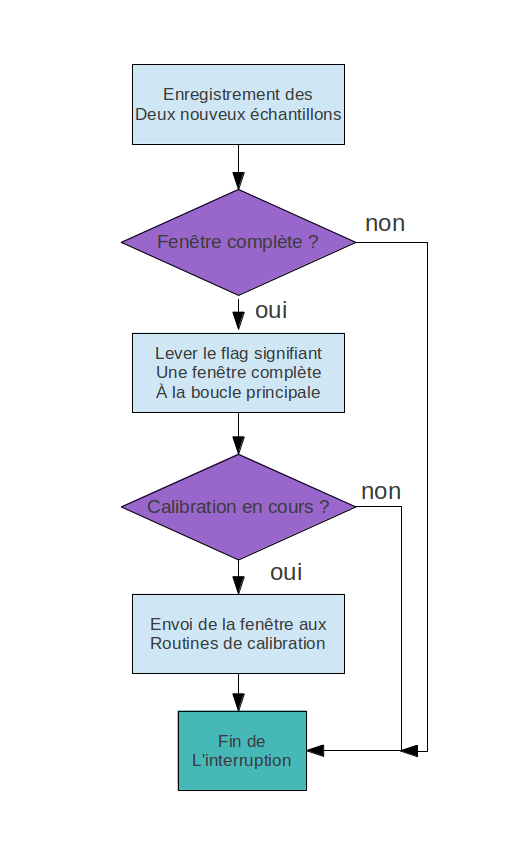
\includegraphics[width=0.6\linewidth]{Figures/adc.png}
	}
	\caption{Routine d'interruption du firmware.}
	\label{fig:adc}
\end{figure}

Il est à noter que deux tableaux de données sont utilisés pour chaque canal. L'un des tableaux est rempli au fur et à mesure par l'ADC pendant que l'autre est traité, c'est à dire filtré puis passé à la détection d'activité. Une fois qu'un tableau est rempli par l'ADC, celui-ci est passé en phase de traitement, et l'autre est rempli à nouveau par l'ADC. Il est donc nécessaire que le tableau à traiter le soit avant qu'une nouvelle fenêtre ne soit acquise, sinon des données seront perdues. 

\subsection{Application de monitorage des signaux}

La partie firmware ayant été présentée, le dernier élément technique du projet est la réalisation du programme de monitorage des signaux. Cette application est un programme tournant sur un ordinateur. L'ordinateur, grâce aux données reçues à travers la liaison série, est en mesure d'afficher les données acquises ou calculées par le PIC32. 

Ceci a été utile lors de la réalisation dans un premier temps à des fins de débogage, puis après pour l'utilisation même du système. En effet, l'interface graphique permet de lancer les phases de calibration du système, pour calibrer les seuils de détection d'activité musculaire, et pour calibrer la bande de base du filtre. 

Ce programme permet également de faire le lien entre le PIC32 et le bras robotique JACO. Cette partie a nécessité l'ajout d'une sur-couche logicielle supplémentaire pour cause d'incompatibilité de langages comme le présentera la partie \ref{CHMono}.

Enfin la conception complète, à savoir le diagramme UML du programme ainsi que son algorithme principal seront détaillés, ainsi que toute les fonctionnalités finales du programme.

\subsubsection{Choix des Librairies et des langages}

Le choix des langages de programmation ont été effectués au début du projet. En lisant la documentation fournie par Kinova, il s'est avéré possible d'interfacer Jaco avec un programme C++. De plus, l'état de l'art de la robotique moderne utilise largement le langage C++, qui en est devenu un des standards. 

En effet, le framework open source ROS (Robot Operating System) est intégralement développé en C++ et Python, deux langages facilement interfaçables. 

La librairie Qt est une librairie graphique libre qui permet la création facile et multi plateforme d'interfaces graphiques robustes. Cette librairie est l'une des plus complète existant aujourd'hui et possède des modules supplémentaires multi plateforme en grand nombre, comme un module réseau, des bases de données, la gestion des fichiers ou encore l'utilisation d'architectures modèle-vue déjà implémentées. Ceci permet d'ouvrir beaucoup d'options pour la suite du développement du projet, dans le cas où de nouveaux éléments viendraient à y être ajoutés. 

La combinaison de ces arguments a donc logiquement tourné le choix du langage informatique principal du programme vers le langage C++.

Cependant, après plusieurs mois de développement, il s'est avéré que l'utilisation des librairies de Kinova doive se faire en passant par une couche logicielle supplémentaire : Mono. Cette partie est détaillée dans la partie suivante.

En effet, les librairies de Kinova ont été nativement réalisée en langage C\#. Le C\# est un langage développé par Microsoft et qui est de ce fait, conçu pour fonctionner de manière optimale sous Windows. Afin d'augmenter les possibilités de développement en C\#, une librairie a été conçue par la communauté open source afin de rendre le C\# utilisable sur d'autres systèmes d'exploitation comme linux ou MacOS.  

\subsubsection{Lien avec Jaco et Mono}\label{CHMono}

Le but du projet étant de contrôler le bras JACO, il est nécessaire d’utiliser l’interface de programmation (API) de Kinova pour le contrôler. Cette librairie permet la connexion du bras JACO au programme via USB, et implémente toutes les méthodes permettant d'envoyer des ordres précis à JACO. Ces ordres peuvent être des ordres de configuration du bras, ou bien des commandes pour lire des valeurs d'état du bras (courant dans les articulation, température des moteurs, angles des articulations, ...), des commandes de déplacements des articulations, ou mêmes des trajectoires de mouvement. 

L’API Kinova a été réalisée intégralement en C\#, et est donc inutilisable directement par un programme codé en C++ pur. Dans sa documentation, Kinova préconise l'utilisation d'un framework appelé Mono pour l'utiliser depuis un programme C++.

Mono est une librairie permettant de mettre a disposition des structures de données (classes, fonctions… ) du monde C++ accessibles au monde .NET (C\#) et inversement. De ce fait, un programme C++ peut déclarer des objets définis en C\# et utiliser ses méthodes.

Le monde .NET permet de créer, à la compilation un type de fichiers appelés des Assembly. Ce sont des fichiers de type .exe ou .dll directement générés par du C\#. Dans le cas du système, le but est d’avoir accès au code contenu dans les fichiers dll de Kinova.

L’API kinova est constituée de sept DLL regroupant diverses classes et fonctions utiles à l’utilisation de JACO. Plutôt que d’importer les 7 dll de kinova dans mono, et de devoir aller chercher chaque classe ou fonction dans le bon Assembly, il a été conseillé par un ingénieur Kinova d'encapsuler toutes les
classes et fonctions requises et de générer une nouvelle DLL unique regroupant toutes ces fonctions. Cela permet de n'appeler qu'un seul fichier .dll ne contenant uniquement que les fonctions et classes dont on a besoin pour la réalisation du système. Cela permet un code beaucoup plus propre et beaucoup moins lourd à réaliser tant qu’à assimiler.

On crée ensuite une classe JACO en C++. Cette classe propose toutes les méthodes de la classe C\# de l'API Kinova. Toute fois, les méthodes de cette classe contiennent les appels aux fonctions C\# grâce à Mono. De cette manière, JACO est interfacé comme une classe normale, et aucun code concernant Mono ne sort de cette classe. 

Tous ces étages réalisés permettent de faire abstraction de toute la partie gérée par Mono et d’utiliser l’API de Kinova comme si celle-ci était accessible directement en C++. Le schéma \ref{fig:mono} résume l'utilisation des librairie Kinova dans le système.

\begin{figure}
	\centering
	\fbox{
		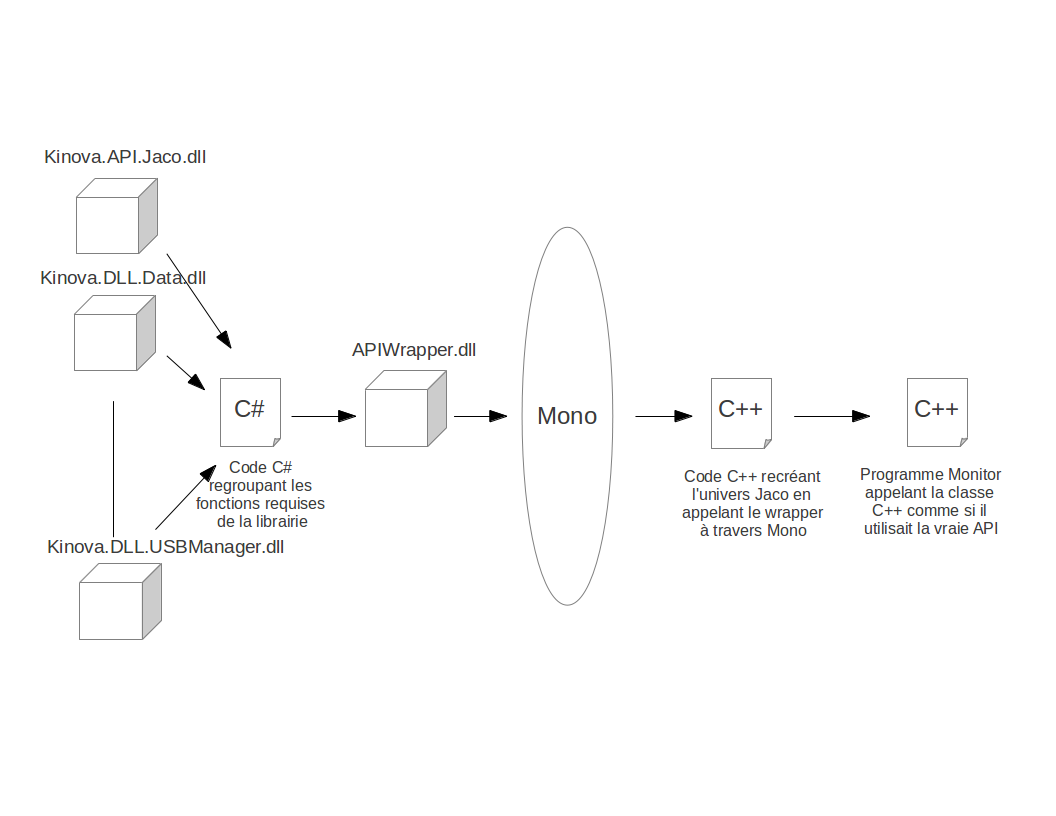
\includegraphics[width=0.8\linewidth]{Figures/mono.png}
	}
	\caption{Interfaçage de l'API Kinova à travers Mono.}
	\label{fig:mono}
\end{figure}

En synthétisant :
\begin{itemize}
 \item On écrit un programme C\# regroupant toutes les fonctions de la librairie Kinova dont ont a besoin. Ce programme fait appel directement aux fichiers .dll fournis par Kinova. 
 \item On construit un nouvel assembly : APIWrapper.dll qui sera appelé dans le programme de monitorage
 \item Grâce à Mono, on charge les classes et méthode de APIWrapper dans le programme C++ grâce à une classe Jaco
 \item Le programme se connecte à Jaco en appelant les méthodes de la classe Jaco
\end{itemize}

\subsubsection{Fonctionnement Global et Schéma UML du Projet}

Le logiciel de monitorage des signaux est un programme basé autour de l'interface graphique réalisée grâce à la librairie Qt. Le diagramme UML du programme est présenté par la figure \ref{fig:uml}.

\begin{figure}
	\centering
	\fbox{
		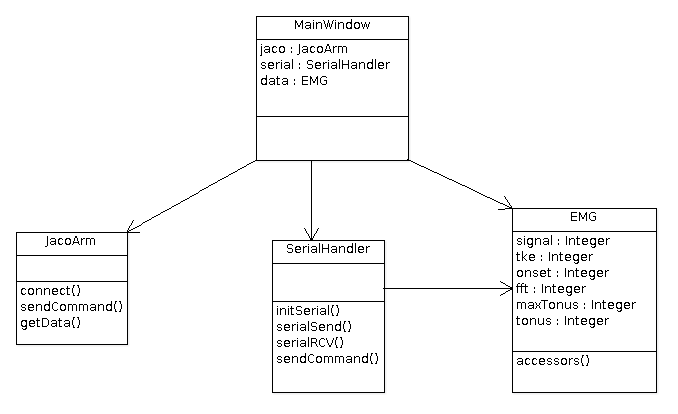
\includegraphics[width=0.8\linewidth]{Figures/ClassDiagram.png}
	}
	\caption{Diagramme UML du programme de monitoring.}
	\label{fig:uml}
\end{figure}

MainWindow est la classe principale de l'interface graphique, c'est elle qui contient tous les éléments graphiques de l'interface. Elle dialogue avec les autres classes afin d'en afficher les données entrantes et sortantes. 

La classe SerialHandler est l'objet qui gère tout ce qui touche à la communication série. Elle possède une méthode de réception des données qui tourne dans un processus séparé du reste du programme.

La classe EMG est la classe contenant toutes les données EMG reçues du PIC32. Lorsqu'une donnée est reçue, elle est réceptionnée par l'objet SerialHandler qui met à jour les données dans la classe EMG. MainWindow va ensuite chercher les données dans la classe EMG afin de les afficher dans l'interface. 

La classe JacoArm est la classe décrite dans la partie précédente qui fait le lien avec les méthodes des librairies de Kinova à travers Mono. C'est dans cette classe que Mono est utilisé.

L'interface graphique réalisée possède plusieurs onglet permettant chacun de visualiser un signal pour les quatre canaux. La figure \ref{fig:gui1} montre la fenêtre de visualisation des signaux EMG pour les quatre canaux. Un autre onglet permet de visualiser le TKE, un autre la détection d'activité musculaire et un dernier permet de monitorer une fft. 

Deux onglet supplémentaires viennent s'ajouter aux quatre onglets de visualisation des signaux. Le premier, présenté par la figure \ref{fig:gui2} permet le contrôle de Jaco. En effet, Jaco étant normalement contrôlé par son joystick, il faut donc activer ou désactiver son contrôle par l'API. Cette fenêtre permet également de visualiser le statut de cette connexion et de visualiser les informations renvoyées par Jaco. 

Enfin le dernier onglet présenté sur la figure \ref{fig:gui3} permet d'envoyer les commandes de calibration au PIC32. Ces calibrations sont la calibration du tonus au repos, du tonus maximum et de la bande de base pour le filtre, et ce pour chaque canal EMG.

%TODO rajouter les deux figures manquantes.

\begin{figure}
	\centering
	\fbox{
		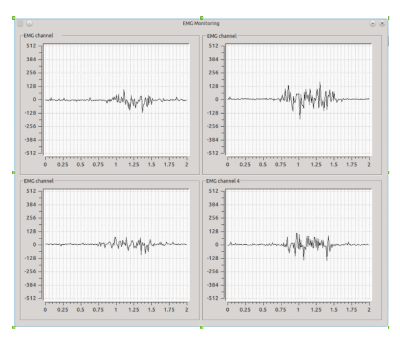
\includegraphics[width=0.8\linewidth]{Figures/gui1.png}
	}
	\caption{Capture d'écran de l'interface graphique du programme de monitorage des données EMG.}
	\label{fig:gui1}
\end{figure}

\begin{figure}
	\centering
	\fbox{
		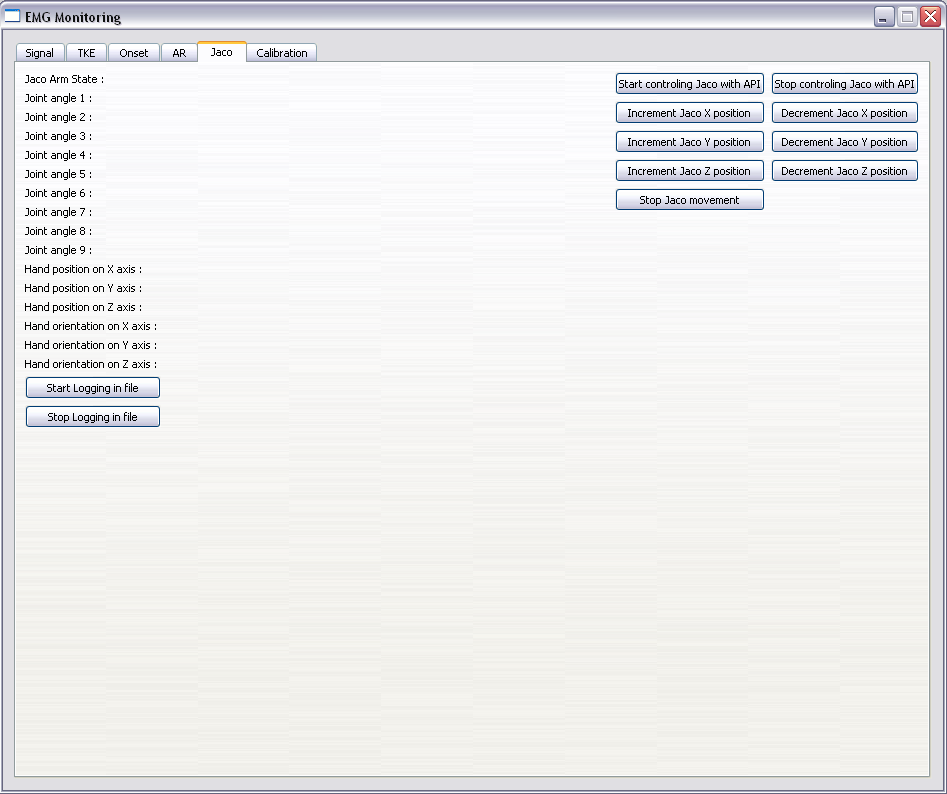
\includegraphics[width=0.8\linewidth]{Figures/gui2.png}
	}
	\caption{Capture d'écran de l'interface graphique du programme de monitorage des données EMG.}
	\label{fig:gui2}
\end{figure}

\begin{figure}
	\centering
	\fbox{
		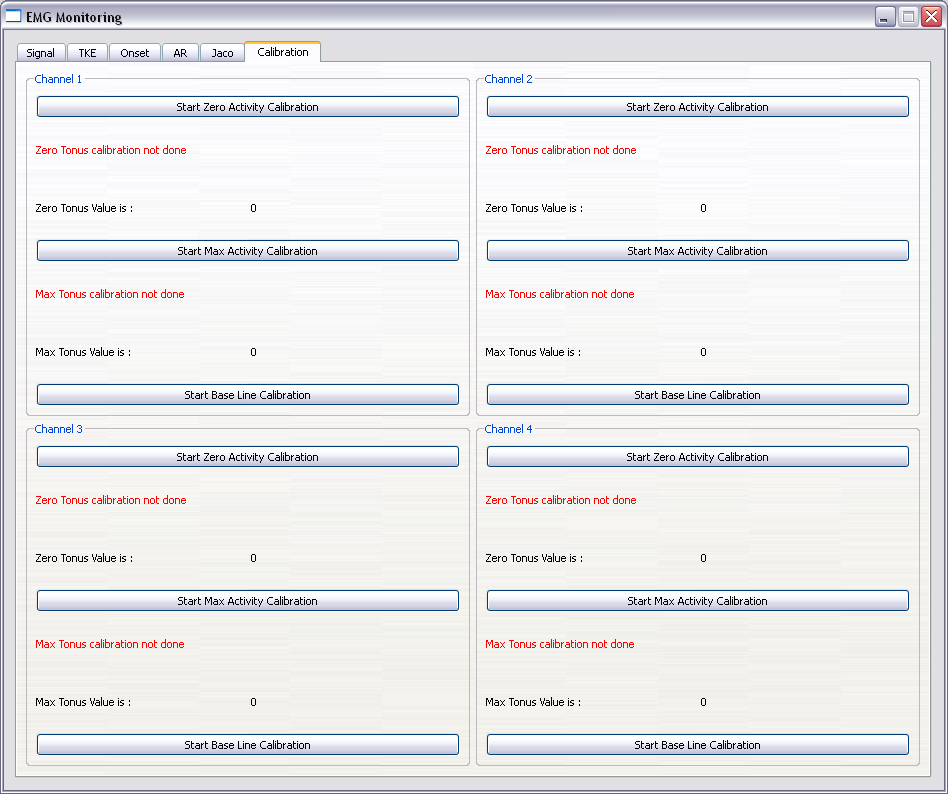
\includegraphics[width=0.8\linewidth]{Figures/gui3.png}
	}
	\caption{Capture d'écran de l'interface graphique du programme de monitorage des données EMG.}
	\label{fig:gui3}
\end{figure}


\section{Validation du Système}

Le système ayant maintenant été décrit dans son ensemble, il est maintenant important de présenté la manière utilisée pour valider ses performance sur un utilisateur. La partie suivante présente le protocole de validation de performances du système tel qu'il a été présenté en commité d'éthique en mai 2013, et présente les expérimentation prévues.

\subsection{Protocole de validation}

\subsubsection{Mode de recrutement} 

Les participants seront recrutés par affichage au sein du laboratoire de recherche de recherche en imagerie et orthopédie ainsi que dans le département de génie de la production automatisée. Ils devront répondre aux critères suivants : 

\begin{itemize}
 \item Critères d'inclusion
 \begin{itemize}
 	\item Les sujets seront des adultes volontaires de plus de 18 ans.
 \end{itemize}
 \item Critères d'exclusion, le sujet de devra pas être sujet à :
  \begin{itemize}
 	\item des douleurs cervicales
 	\item des torticolis fréquents
 	\item tout problème orthopédique de la ceinture scapulaire et cervicale
 	\item des maux de tête réguliers
 \end{itemize}
\end{itemize}


\subsubsection{Principe de fonctionnement}

La détection de l’activité musculaire se fera par un seuil appliqué sur l’énergie du signal  (TKE) du signal EMG échantillonné à 2KHz. Le but de ce protocole est de déterminer la sensibilité du système en le testant sur 10 sujets. L’activité musculaire générée lors d’un mouvement dépend de l’amplitude du mouvement effectué, ainsi que de la vitesse à laquelle le mouvement est effectué. Ainsi la validation s’effectuera en faisant effectuer au sujet plusieurs mouvements d’amplitudes différentes à des vitesses différentes. 

\subsubsection{Protocole expérimental}

Un capteur inertiel (Interlink, Microstrain) sera utilisé afin d’enregistrer l’angle de rotation de la tête ainsi que la vitesse angulaire du mouvement. Celui-ci sera disposé sur un casque de type casque d’écoute audio avec les oreilles comme point de repère de placement. 

Un pointeur laser sera également disposé sur la tête du sujet afin que celui-ci puisse indiquer au sujet l’orientation précise de sa tête.
 
L’angle visé sera indiqué au sujet par des marqueurs disposés devant lui et vers lesquels il devra tourner la tête en se repérant à l’aide du pointeur laser. La vitesse visée sera indiquée au sujet par le biais d’un métronome électronique. Le sujet devra réaliser le mouvement vers le marqueur indiqué en un temps de métronome. 

La figure \ref{fig:rotationtete} décrit l'angle de rotation de la tête à effectuer par le sujet.

\begin{figure}
	\centering
	\fbox{
		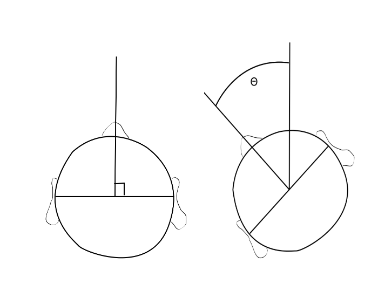
\includegraphics[width=0.6\linewidth]{Figures/rotationtete.png}
	}
	\caption{Description de l'angle de rotation de la tête.}
	\label{fig:rotationtete}
\end{figure}

\subsubsection{Déroulement des acquisitions}

Le sujet sera assis devant une surface comportant les cibles qu’il devra viser avec le pointeur laser. Le pointeur laser ainsi que le capteur angulaire seront disposés sur un casque d’écoute audio qui sera placé sur les oreilles du sujet.
Une étape de familiarisation au métronome et d’entrainement à la visée permettra au sujet de s’entrainer à effectuer le mouvement aux angles prévus à la bonne vitesse.

Voici une liste des mesures qui seront prises pendant l’expérimentation : 

\begin{itemize}
 \item Angle de rotation de la tête 
 \item Vitesse angulaire de rotation de la tête 
 \item Signaux électromyographique du muscle sterno-cléïdo mastoïdien
 \item Signal de détection d’activité musculaire
\end{itemize}

Et ce pour chaque combinaison d’angle et de vitesse de métronome ciblés.

Le sujet devra réaliser des mouvements de rotation de la tête à des angles de $10$ degrés, $20$ degrés, $30$ degrés, $40$ degrés, $50$ degrés, $60$ degrés, $70$ degrés et $80$ degrés. Chaque déplacement angulaire sera effectué à des vitesses de métronomes de $60 bpm, 90 bpm, 120 bpm, 160 bpm$ et $200 bpm$ (battement par minute) . 

L’ordre des vitesses et des angles sera tiré au hasard avant l’expérimentation pour chaque sujet.

\subsubsection{Notes importantes}

Après chaque mouvement un fichier devra être sauvé sous la forme aXXvYYY.csv où XX correspond a la valeur de l’angle visé lors de l’enregistrement et YYY correspond à la valeur du métronome utilisé pour l’enregistrement.

A chaque acquisition, un monitoring sera effectué sur le programme Monitor afin de vérifier si le système a détecté une activité musculaire ou non. Le fichier de sauvegarde devra être sauvegardé dans le même dossier que les données du capteur angulaire sous la forme emgaXXvYYY.txt

\subsubsection{Exemple de données récoltées}

Les figures \ref{fig:validExAng}, \ref{fig:validExEMG}, \ref{fig:validExVit} et \ref{fig:validExOnset} montrent un exemple de la forme que prendront les données récoltées lors d’une acquisition sur une personne : (A20, A30, A40, A50, A60 correspondent à l’angle de rotation effectué, et V60, V90, V120, V160 et V200 correspondent aux vitesses du métronome pour l’acquisition)

\begin{figure}
	\begin{minipage}{0.40\textwidth}
		\fbox{
			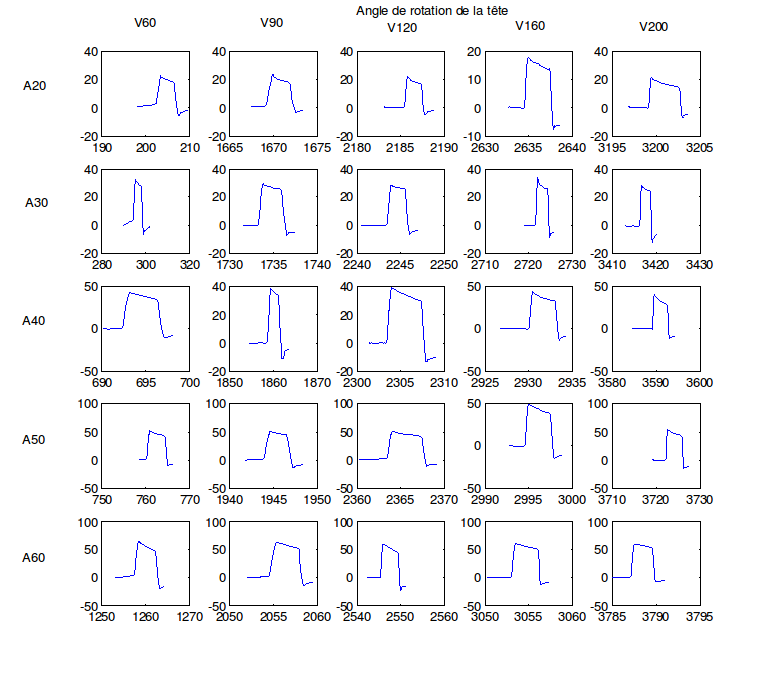
\includegraphics[width=\textwidth]{Figures/validExAngle.png}
		}
		\caption{Exemple de données d'angles de rotation de la tête}
		\label{fig:validExAng}
	\end{minipage}
	\hspace{0.1\textwidth}
	\begin{minipage}{0.40\textwidth}
		\fbox{
			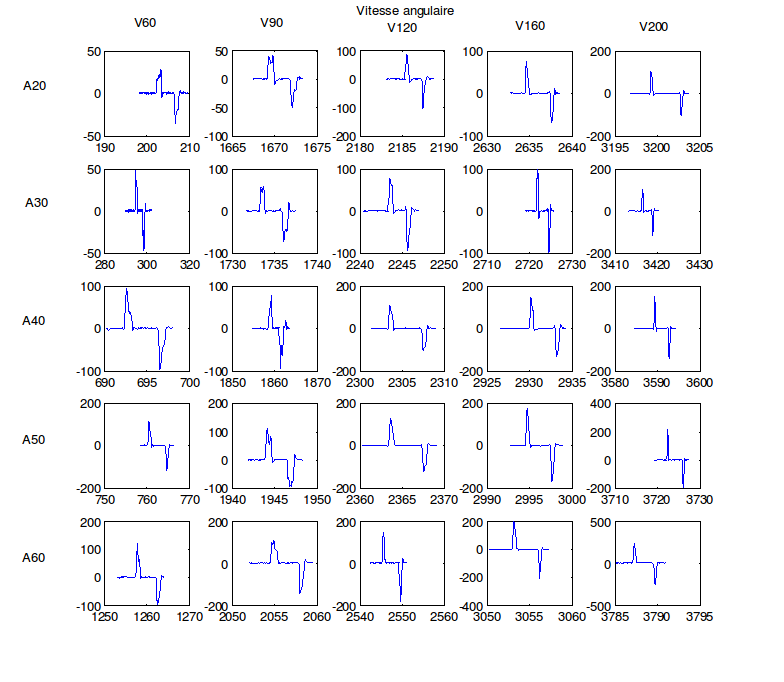
\includegraphics[width=\textwidth]{Figures/validExVit.png}
		}
		\caption{Exemple de données de vitesse anglulaires de rotation de la tête}
		\label{fig:validExVit}
	\end{minipage}
	\vspace*{20mm}
	\begin{minipage}{0.40\textwidth}
		\fbox{
			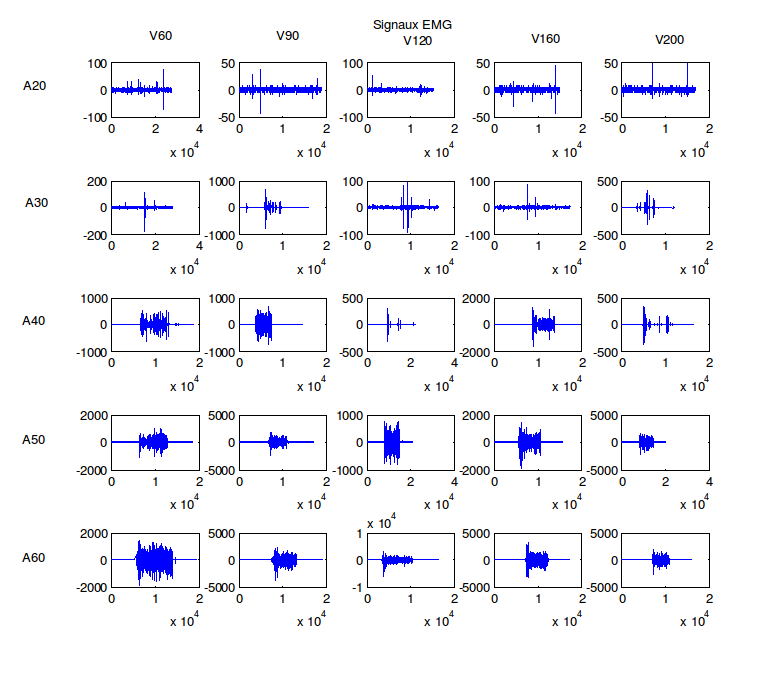
\includegraphics[width=\textwidth]{Figures/validExEMG.png}
		}
		\caption{Exemple de données d'EMG de rotation de la tête}
		\label{fig:validExEMG}
	\end{minipage}
	\hspace{0.1\textwidth}
	\begin{minipage}{0.40\textwidth}
		\fbox{
			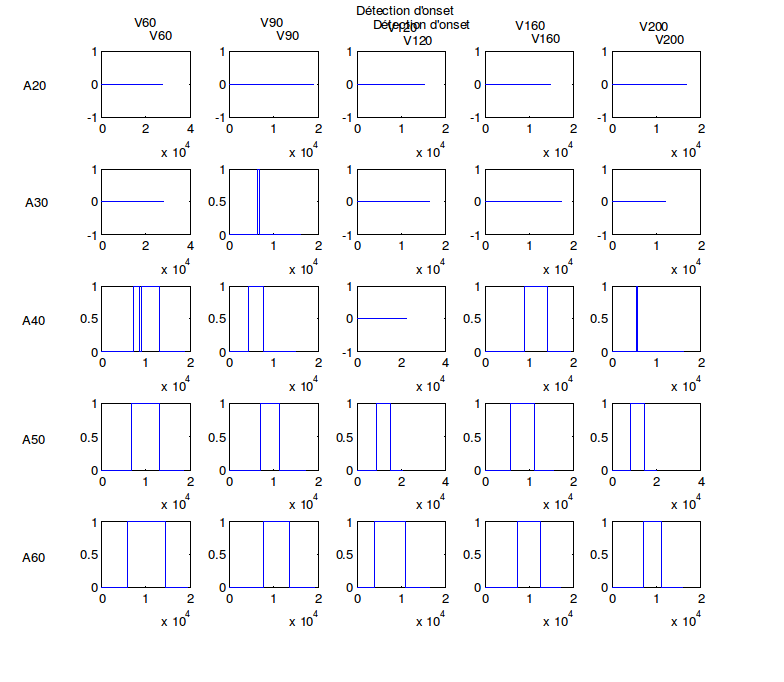
\includegraphics[width=\textwidth]{Figures/validExOnset.png}
		}
		\caption{Exemple de données de détection d'activité }
		\label{fig:validExOnset}
	\end{minipage}
\end{figure}


Ces données représentent les valeurs brutes enregistrées grâce aux capteurs inertiel et EMG. 

\subsubsection{Interprétation des données}

Une fois les données acquises, 4 paramètres seront estimés pour évaluer la sensibilité du système correspondant au sujet testé : l’efficacité, le coefficient de l’angle maximum, le coefficient de la vitesse angulaire maximale ainsi que l’efficacité globale.

Le paramètre de l’efficacité est définit comme le rapport entre le nombre de détections sur le nombre d’essais total comme montré par l'équation \ref{eq:validEff}.

\begin{align}\label{eq:validEff}
   Efficacite = \frac{Nb\ de\ détections}{Nb\ d'essais\ total} 
\end{align}

On est en mesure de donner une valeur entre 0 et 1 à l’efficacité du système pour une personne donnée. La valeur 1 indique que le système a détecté toutes les activités réalisées par la personne et la valeur 0 indique au contraire que le système n’en a détecté aucune. 

Cependant ce paramètre ne prend pas en compte les angles et vitesses angulaires atteintes lors des expérimentations. On détermine donc un coefficient d’angle ainsi qu’un coefficient de vitesse angulaire, qui viendront pondérer le coefficient d’efficacité de chaque sujet. Ces coefficients seront basés sur l’angle maximum atteint par un sujet et la vitesse angulaire atteinte par un sujet. Ainsi les résultats seront pondérés relativement au sujet ayant atteint l’angle et la vitesse angulaire les plus grands. 

Ainsi on fixe un angle maximum égal au plus grand atteint par un sujet, ce sujet aura un coefficient d’angle de 1. Les autres auront un coefficient défini comme le définit l'équation \ref{eq:validCoeffAng}. 

\begin{align}\label{eq:validCoeffAng}
   Coeff_{angle} = \frac{Angle\ max\ du\ sujet}{Angle\ max\ atteint\ par\ un\ sujet} 
\end{align}

De la même manière un coefficient de vitesse angulaire sera appliqué. On fixe une vitesse angulaire maximum atteinte par un sujet, celui-ci aura un coefficient de vitesse angulaire de 1. Les autres auront un coefficient défini comme le définit l'équation \ref{eq:validCoeffVit}.

\begin{align}\label{eq:validCoeffVit}
   Coeff_{vitesse} = \frac{Vitesse\ angulaire\ max\ du\ sujet}{Vitesse\ angulaire\ max\ atteint\ par\ un\ sujet} 
\end{align}

Cela nous permet donc de fixer une efficacité globale pour chaque sujet qui sera calculée à partir de l’équation suivante : 


\subsubsection{Comparaison des données}

Les valeurs d’efficacité globale de chaque sujet seront mises en commun et comparées les unes aux autres afin de savoir si le système fonctionne de manière similaire sur plusieurs personnes ou si ses performances sont variables d’une personne à l’autre.
Une personne ayant une détection d’activité de $100\%$ aura une efficacité de 1, une personne ayant une détection d’activité de $0\%$ aura une efficacité de 0. Ainsi, plus un score d’efficacité est bon, plus il est proche de 1.
Une efficacité moyenne, ainsi qu’une efficacité globale moyenne pourront être déterminées ainsi que leurs écarts types. Un seuil supérieur ou égal à la valeur de $0.75$ pour l’efficacité globale permettra d’indiquer que le système est acceptable. En comparant les performances des sujets, si un sujet obtient un score plus faible que les autres, les données nous permettront d’en étudier les causes, et permettront potentiellement de trouver des pistes d’amélioration du système.

\chapter{Résultats}

\section{Détection d'activité}

\section{Temps de calcul et chronogrammes}

\section{Validation du système}

\chapter{Discussion}

\begin{conclusion}
Texte de conclusion

\end{conclusion}


%%%%%%%%%%%%%%%%%%%%%%%%%%%%%%%%%%%%%%%%%%%%%%%%%%%
%  ANNEXE:
%%%%%%%%%%%%%%%%%%%%%%%%%%%%%%%%%%%%%%%%%%%%%%%%%%%
\appendix


\multiannexe % si on a plus d'une annexe
%\include{annexe1}
\chapter{Titre de l'annexe} 

S'il y lieu

\section{Première Section de l'Annexe}
<Texte à inserer> 

Lorem ipsum dolor sit amet, consectetur adipiscing elit. Pellentesque justo justo, porta sagittis feugiat eget, ornare rhoncus ligula. Nunc non odio sed lacus rutrum rhoncus. Mauris non congue arcu. Cras quis quam tortor. In ultrices tincidunt magna sed suscipit. Curabitur vel tellus sapien, ut tincidunt arcu. Maecenas dapibus ullamcorper urna, ut mollis mi tincidunt a. Nam eu orci nec lacus consectetur commodo. Donec purus tellus, consectetur at feugiat quis, scelerisque congue nibh. Aliquam urna dolor, congue nec euismod eget, convallis vitae libero. Sed vel magna suscipit leo suscipit porta quis et nunc. Nullam ante tellus, tincidunt a fringilla vel, rutrum non tellus. In volutpat consectetur purus, in euismod lorem feugiat vel. Aliquam sodales nisl eget sapien ullamcorper posuere consectetur orci bibendum. Vestibulum pulvinar viverra auctor. Vivamus ac sem et enim sodales dictum. Test citation \cite{Bha10}

Tests de figure en annexe.

%%%%%%%%%%%%%%%%%%%%%%%%%%%%%%%%%%%%%%%%%%%%%%%%%%%%%%%%%%%%%%%%%%%%%
% On a crée les environiments figurep et tablep pour que les figures et
% les tableaux de l'annexe n'apparaissent pas dans les listes de figures et tableaux
%

\begin{figureap}[ht]
	\fbox{ % cette commande est nécéssaire pour encadrer les figures
	\centering
		
\includegraphics{Figures/logoets.jpg}
	}
	\caption{Logo de l'ÉTS dans l'annexe. Ici on va mettre un peu plus de texte pour voir comment va être la présentation de
	la légende dans ce cas.}
	\label{fig:testap}
\end{figureap}
\begin{center}
\begin{equation} 
2*x=4 
\end{equation}
\end{center}

\begin{tableap}[*ht]
	\caption{Un autre tableau. Ici on va rédiger un peu plus de texte pour vérifier si la légende sera bien placé.}
		\begin{tabular}{|c|c|c|c|c|c|c|c|}
		\hline
			{\bf titre} & {\bf titre} & {\bf titre} & {\bf titre} & {\bf titre} & {\bf titre} & {\bf titre} & {\bf titre} \\
	  \hline
			blá & blá & blá & blá & blá & blá & blá & blá \\
	  \hline
			blá & blá & blá & blá & blá & blá & blá & blá \\
	  \hline
			blá & blá & blá & blá & blá & blá & blá & blá \\
	  \hline
			blá & blá & blá & blá & blá & blá & blá & blá \\
	  \hline
			blá & blá & blá & blá & blá & blá & blá & blá \\
	  \hline
			blá & blá & blá & blá & blá & blá & blá & blá \\
	  \hline
		\end{tabular}
	\label{tab:tableau_annexe}
\end{tableap}

Test citation \ref{fig:testap}.

Lorem ipsum dolor sit amet, consectetur adipiscing elit. Pellentesque justo justo, porta sagittis feugiat eget, ornare rhoncus ligula. Nunc non odio sed lacus rutrum rhoncus. Mauris non congue arcu. Cras quis quam tortor. In ultrices tincidunt magna sed suscipit. Curabitur vel tellus sapien, ut tincidunt arcu. Maecenas dapibus ullamcorper urna, ut mollis mi tincidunt a. Nam eu orci nec lacus consectetur commodo. Donec purus tellus, consectetur at feugiat quis, scelerisque congue nibh. Aliquam urna dolor, congue nec euismod eget, convallis vitae libero. Sed vel magna suscipit leo suscipit porta quis et nunc. Nullam ante tellus, tincidunt a fringilla vel, rutrum non tellus. In volutpat consectetur purus, in euismod lorem feugiat vel. Aliquam sodales nisl eget sapien ullamcorper posuere consectetur orci bibendum. Vestibulum pulvinar viverra auctor. Vivamus ac sem et enim sodales dictum.
\begin{equation}
x = 42
\end{equation} 
Lorem ipsum dolor sit amet, consectetur adipiscing elit. Pellentesque justo justo, porta sagittis feugiat eget, ornare rhoncus ligula. Nunc non odio sed lacus rutrum rhoncus. Mauris non congue arcu. Cras quis quam tortor. In ultrices tincidunt magna sed suscipit. Curabitur vel tellus sapien, ut tincidunt arcu. Maecenas dapibus ullamcorper urna, ut mollis mi tincidunt a. Nam eu orci nec lacus consectetur commodo. Donec purus tellus, consectetur at feugiat quis, scelerisque congue nibh. Aliquam urna dolor, congue nec euismod eget, convallis vitae libero. Sed vel magna suscipit leo suscipit porta quis et nunc.

\subsection{Test}


Lorem ipsum dolor sit amet, consectetur adipiscing elit. Pellentesque justo justo, porta sagittis feugiat eget, ornare rhoncus ligula. Nunc non odio sed lacus rutrum rhoncus. Mauris non congue arcu. Cras quis quam tortor. In ultrices tincidunt magna sed suscipit. Curabitur vel tellus sapien, ut tincidunt arcu. Maecenas dapibus ullamcorper urna, ut mollis mi tincidunt a. Nam eu orci nec lacus consectetur commodo. Donec purus tellus, consectetur at feugiat quis, scelerisque congue nibh. Aliquam urna dolor, congue nec euismod eget, convallis vitae libero. Sed vel magna suscipit leo suscipit porta quis et nunc. Nullam ante tellus, tincidunt a fringilla vel, rutrum non tellus. In volutpat consectetur purus, in euismod lorem feugiat vel. Aliquam sodales nisl eget sapien ullamcorper posuere consectetur orci bibendum. Vestibulum pulvinar viverra auctor. Vivamus ac sem et enim sodales dictum.

\citerefs{Test} \citerefs{Test2}


%%%%%%%%%%%%%%%%%%%%%%%%%%%%%%%%%%%%%%%%%%%%%%%%%%%
% LISTE DE RÉFERENCES
%
% IMPORTANT:
% Pour que ça marche:
%   1. Compiler le document une fois
%   2. Rouler la commande: << bibtex refs >>...cliquer sur le fichier update_refs.bat sur Windows
%   3. Recompiler le document
%%%%%%%%%%%%%%%%%%%%%%%%%%%%%%%%%%%%%%%%%%%%%%%%%%%

%Changement d'interligne pour passer en simple pour les références et la bibliographie.

%\newpage
\singlespacing
%\nociterefs{*} %Ici vous devez inclure les références qui ne sont pas cités, ou étoiles pour toutes les réfs
\bibliographystylerefs{bibETS}
\addcontentsline{toc}{chapter}{LISTE DE RÉFÉRENCES}
\bibliographyrefs{refs} % à décommanter et indiquer la liste des fichiers bib
\onehalfspacing

%------------------------------------------------------------------------------------------------------------------------------------------


%%%%%%%%%%%%%%%%%%%%%%%%%%%%%%%%%%%%%%%%%%%%%%%%%%%
% BIBLIOGRAPHIE
%%%%%%%%%%%%%%%%%%%%%%%%%%%%%%%%%%%%%%%%%%%%%%%%%%%
\newpage
\singlespacing
%\nocite{*}
\bibliographystyle{bibETS}
\addcontentsline{toc}{chapter}{BIBLIOGRAPHIE}
\bibliography{biblio} % à décommanter et indiquer la liste des fichiers bib
\onehalfspacing

\end{document}
